\documentclass{beamer}
\usetheme[secheader]{Boadilla}

\defbeamertemplate*{footline}{Boadilla}
{
   \leavevmode%
   \hbox{%
%   \begin{beamercolorbox}[wd=.333333\paperwidth,ht=2.25ex,dp=1ex,right]{author in head/foot}%
%     \usebeamerfont{author in head/foot}\insertshortauthor~~(\insertshortinstitute)
%   \end{beamercolorbox}%
%   \begin{beamercolorbox}[wd=.333333\paperwidth,ht=2.25ex,dp=1ex,right]{title in head/foot}%
%     \usebeamerfont{title in head/foot}\insertshorttitle
%   \end{beamercolorbox}%
   \begin{beamercolorbox}[wd=1\paperwidth,ht=2.25ex,dp=1ex,right]{date in head/foot}%
%     \usebeamerfont{date in head/foot}\insertshortdate{}\hspace*{2em}
     \insertframenumber{}\hspace*{2ex}
   \end{beamercolorbox}}%
   \vskip0pt%
}


\usepackage{comment}
% wow this is a hack that lets you have more definitions in latex.
% see http://www.tex.ac.uk/cgi-bin/texfaq2html?label=noroom
\usepackage{natbib}
\usepackage{etex}
\usepackage{pgffor}
\usepackage[utf8]{inputenc}
%\usepackage[cyr]{aeguill}
\reserveinserts{28}
\usepackage{tikz}
\usepackage[customcolors]{hf-tikz}
%\usepackage[utf8]{inputenc}
%\mode<presentation>{\usetheme{Caltech}}

\usepackage{amsmath}
\usepackage{mathtools}
\usepackage{amssymb}
\usepackage{amsfonts}
\usepackage{amsthm}
\usepackage{multimedia}
\usepackage{color}
\usepackage{esint}
\usepackage{stmaryrd}
\usepackage{tabularx}
\usepackage{multirow}
\usepackage[squaren]{SIunits}
\usepackage{graphicx}
\usepackage{diagbox}
\usepackage{pdfpages}
\usepackage{dsfont}
\usepackage{xcolor}
\usepackage{soul}
\usepackage[linesnumbered,ruled,vlined]{algorithm2e}

\usepackage{subfig}

\graphicspath{{./img/}}

\newcommand{\cplus}{\colorbox{green}{($+$)} }
\newcommand{\cmoins}{\colorbox{red}{($-$)} }
\newcommand{\cmean}{\colorbox{yellow}{($\pm$)}}

\newcommand{\mathcolorbox}[2]{\colorbox{#1}{$\displaystyle #2$}}



%%%%%%%%%%%%%%%%%%%%%%%%%%%%
% Paper dependent stuff    %
%%%%%%%%%%%%%%%%%%%%%%%%%%%%


\newcommand{\ov}{\overline}
\newcommand{\oa}{\ov{a}}
%\newcommand{\oQ}{\ov{Q}}
%\newcommand{\oR}{\ov{R}}
\newcommand{\ox}{\ov{x}}
\newcommand{\oz}{\ov{z}}
\newcommand{\oy}{\ov{y}}
\newcommand{\os}{\ov{s}}
%\newcommand{\or}{\ov{r}}
%\newcommand{\ocS}{\ov{\cS}}
\newcommand{\ocF}{\ov{\cF}}
%\newcommand{\augmentedtransition}{\ov{\transition}
%\newcommand{\ocA}{\ov{\cA}}

%%%%%%%%%%%%%%%%%%%%%%%%%%%%rans
% Aesthetics               %
% over-underline, hat, bold%
%%%%%%%%%%%%%%%%%%%%%%%%%%%%

\newcommand{\eps}{\varepsilon}
\newcommand{\vareps}{\varepsilon}
\renewcommand{\epsilon}{\varepsilon}
%\renewcommand{\hat}{\widehat}
\renewcommand{\tilde}{\widetilde}
\renewcommand{\bar}{\overline}

\newcommand*{\MyDef}{\mathrm{\scriptscriptstyle def}}
\newcommand*{\eqdefU}{\ensuremath{\mathop{\overset{\MyDef}{=}}}}% Unscaled version
\newcommand*{\eqdef}{\mathop{\overset{\MyDef}{\resizebox{\widthof{\eqdefU}}{\heightof{=}}{=}}}}


\def\:#1{\protect \ifmmode {\mathbf{#1}} \else {\textbf{#1}} \fi}
\newcommand{\CommaBin}{\mathbin{\raisebox{0.5ex}{,}}}

\newcommand{\wt}[1]{\widetilde{#1}}
\newcommand{\wh}[1]{\widehat{#1}}
\newcommand{\wo}[1]{\overline{#1}}
\newcommand{\wb}[1]{\overline{#1}}

% bf and bm missing due to conflict!!
\newcommand{\bsym}[1]{\mathbf{#1}}
\newcommand{\bzero}{\mathbf{0}}
\newcommand{\ba}{\mathbf{a}}
\newcommand{\bb}{\mathbf{b}}
\newcommand{\bc}{\mathbf{c}}
\newcommand{\bd}{\mathbf{d}}
\newcommand{\be}{\mathbf{e}}
\newcommand{\bg}{\mathbf{g}}
\newcommand{\bh}{\mathbf{h}}
\newcommand{\bi}{\mathbf{i}}
\newcommand{\bj}{\mathbf{j}}
\newcommand{\bk}{\mathbf{k}}
\newcommand{\bl}{\mathbf{l}}
\newcommand{\bn}{\mathbf{n}}
%\newcommand{\bo}{\mathbf{o}}
\newcommand{\bp}{\mathbf{p}}
\newcommand{\bq}{\mathbf{q}}
\newcommand{\br}{\mathbf{r}}
\newcommand{\bs}{\mathbf{s}}
\newcommand{\bt}{\mathbf{t}}
\newcommand{\bu}{\mathbf{u}}
\newcommand{\bv}{\mathbf{v}}
\newcommand{\bw}{\mathbf{w}}
\newcommand{\bx}{\mathbf{x}}
\newcommand{\by}{\mathbf{y}}
\newcommand{\bz}{\mathbf{z}}

\newcommand{\bA}{\mathbf{A}}
\newcommand{\bB}{\mathbf{B}}
\newcommand{\bC}{\mathbf{C}}
\newcommand{\bD}{\mathbf{D}}
\newcommand{\bE}{\mathbf{E}}
\newcommand{\bF}{\mathbf{F}}
\newcommand{\bG}{\mathbf{G}}
\newcommand{\bH}{\mathbf{H}}
\newcommand{\bI}{\mathbf{I}}
\newcommand{\bJ}{\mathbf{J}}
\newcommand{\bK}{\mathbf{K}}
\newcommand{\bL}{\mathbf{L}}
\newcommand{\bM}{\mathbf{M}}
\newcommand{\bN}{\mathbf{N}}
\newcommand{\bO}{\mathbf{O}}
\newcommand{\bP}{\mathbf{P}}
\newcommand{\bQ}{\mathbf{Q}}
\newcommand{\bR}{\mathbf{R}}
\newcommand{\bS}{\mathbf{S}}
\newcommand{\bT}{\mathbf{T}}
\newcommand{\bU}{\mathbf{U}}
\newcommand{\bV}{\mathbf{V}}
\newcommand{\bW}{\mathbf{W}}
\newcommand{\bX}{\mathbf{X}}
\newcommand{\bY}{\mathbf{Y}}
\newcommand{\bZ}{\mathbf{Z}}

% calligraphic
\newcommand{\cf}{\mathcal{f}}
%\newcommand{\cA}{\mathcal{A}}
\newcommand{\cB}{\mathcal{B}}
\newcommand{\cC}{\mathcal{C}}
%\newcommand{\cD}{\mathcal{D}}
\newcommand{\cE}{\mathcal{E}}
\newcommand{\cF}{\mathcal{F}}
\newcommand{\cG}{\mathcal{G}}
\newcommand{\cH}{\mathcal{H}}
\newcommand{\cI}{\mathcal{I}}
\newcommand{\cJ}{\mathcal{J}}
\newcommand{\cL}{\mathcal{L}}
%\newcommand{\cM}{\mathcal{M}}
\newcommand{\cN}{\mathcal{N}}
\newcommand{\cO}{\mathcal{O}}
\newcommand{\cP}{\mathcal{P}}
\newcommand{\cQ}{\mathcal{Q}}
%\newcommand{\cR}{\mathcal{R}}
%\newcommand{\cS}{\mathcal{S}}
\newcommand{\cT}{\mathcal{T}}
%\newcommand{\cU}{\mathcal{U}}
\newcommand{\cV}{\mathcal{V}}
\newcommand{\cW}{\mathcal{W}}
\newcommand{\cX}{\mathcal{X}}
\newcommand{\cY}{\mathcal{Y}}
\newcommand{\cZ}{\mathcal{Z}}

\newcommand{\rf}{\mathscr{f}}
\newcommand{\rA}{\mathscr{A}}
\newcommand{\rB}{\mathscr{B}}
\newcommand{\rC}{\mathscr{C}}
\newcommand{\rD}{\mathscr{D}}
\newcommand{\rE}{\mathscr{E}}
\newcommand{\rF}{\mathscr{F}}
\newcommand{\rG}{\mathscr{G}}
\newcommand{\rH}{\mathscr{H}}
\newcommand{\rI}{\mathscr{I}}
\newcommand{\rJ}{\mathscr{J}}
\newcommand{\rK}{\mathscr{K}}
\newcommand{\rL}{\mathscr{L}}
\newcommand{\rM}{\mathscr{M}}
\newcommand{\rN}{\mathscr{N}}
\newcommand{\rO}{\mathscr{O}}
\newcommand{\rP}{\mathscr{P}}
\newcommand{\rQ}{\mathscr{Q}}
\newcommand{\rR}{\mathscr{R}}
\newcommand{\rS}{\mathscr{S}}
\newcommand{\rT}{\mathscr{T}}
\newcommand{\rU}{\mathscr{U}}
\newcommand{\rV}{\mathscr{V}}
\newcommand{\rW}{\mathscr{W}}
\newcommand{\rX}{\mathscr{X}}
\newcommand{\rY}{\mathscr{Y}}
\newcommand{\rZ}{\mathscr{Z}}

\newcommand{\bbf}{\mathbb{f}}
\newcommand{\bbA}{\mathbb{A}}
\newcommand{\bbB}{\mathbb{B}}
\newcommand{\bbC}{\mathbb{C}}
\newcommand{\bbD}{\mathbb{D}}
\newcommand{\bbE}{\mathbb{E}}
\newcommand{\bbF}{\mathbb{F}}
\newcommand{\bbG}{\mathbb{G}}
\newcommand{\bbH}{\mathbb{H}}
\newcommand{\bbI}{\mathbb{I}}
\newcommand{\bbJ}{\mathbb{J}}
\newcommand{\bbK}{\mathbb{K}}
\newcommand{\bbL}{\mathbb{L}}
\newcommand{\bbM}{\mathbb{M}}
\newcommand{\bbN}{\mathbb{N}}
\newcommand{\bbO}{\mathbb{O}}
\newcommand{\bbP}{\mathbb{P}}
\newcommand{\bbQ}{\mathbb{Q}}
\newcommand{\bbR}{\mathbb{R}}
\newcommand{\bbS}{\mathbb{S}}
\newcommand{\bbT}{\mathbb{T}}
\newcommand{\bbU}{\mathbb{U}}
\newcommand{\bbV}{\mathbb{V}}
\newcommand{\bbW}{\mathbb{W}}
\newcommand{\bbX}{\mathbb{X}}
\newcommand{\bbY}{\mathbb{Y}}
\newcommand{\bbZ}{\mathbb{Z}}


%%%%%%%%%%%%%%%%%%%%%%%%%%%%
% Math jargon              %
%%%%%%%%%%%%%%%%%%%%%%%%%%%%
\newcommand{\wrt}{w.r.t.\xspace}
\newcommand{\defeq}{\stackrel{\mathclap{\normalfont\mbox{\scriptscriptstyle def}}}{=}}
\newcommand{\maxund}[1]{\max\limits_{#1}}
\newcommand{\supund}[1]{\text{sup}\limits_{#1}}
\newcommand{\minund}[1]{\min\limits_{#1}}
\renewcommand{\epsilon}{\varepsilon}
\newcommand{\bigotime}{\mathcal{O}}


\DeclareMathOperator*{\argmin}{arg\,min} 
\DeclareMathOperator*{\argmax}{arg\,max} 
\DeclareMathOperator*{\cupdot}{\mathbin{\mathaccent\cdot\cup}}

%%%%%%%%%%%%%%%%%%%%%%%%%%%%
% Matrix operators         %
%%%%%%%%%%%%%%%%%%%%%%%%%%%%
\newcommand{\transp}{\mathsf{\scriptscriptstyle T}}

%%%%%%%%%%%%%%%%%%%%%%%%%%%%
% Statistic operators      %
%%%%%%%%%%%%%%%%%%%%%%%%%%%%
\newcommand{\probability}[1]{\mathbb{P}\left(#1\right)}
\newcommand{\probdist}{Pr}
\DeclareMathOperator*{\expectedvalue}{\mathbb{E}}
\DeclareMathOperator*{\variance}{\text{Var}}
\newcommand{\expectedvalueover}[1]{\expectedvalue\limits_{#1}}
\newcommand{\condbar}{\;\middle|\;}
\newcommand{\gaussdistr}{\mathcal{N}}
\newcommand{\uniformdistr}{\mathcal{U}}
\newcommand{\bernoullidist}{\mathcal{B}}

%%%%%%%%%%%%%%%%%%%%%%%%%%%%
% Algebraic Sets           %
%%%%%%%%%%%%%%%%%%%%%%%%%%%%
\newcommand{\Real}{\mathbb{R}}
\newcommand{\Natural}{\mathbb{N}}
\newcommand{\statespace}{\mathcal{X}}
\newcommand{\funcspace}{\mathcal{F}}
\newcommand{\dynaspace}{\mathcal{T}}


%\newtheorem{theorem}{Theorem}
%\newtheorem{definition}{Definition}
%\newtheorem{lemma}{Lemma}
%\newtheorem{proposition}{Proposition}
%\newtheorem{remark}{Remark}
%\newtheorem{property}{Property}
%\newtheorem{assumption}{Assumption}
%\newtheorem{conjecture}{Conjecture}


%\input{../glossary.tex}
\newcommand{\Q}{Q}
\newcommand{\V}{V}
\newcommand{\mubot}{\mu_{\bot}}
\newcommand{\mutop}{\mu_{\top}}
\newcommand{\params}{\theta}
\newcommand{\dirac}{\delta}
\newcommand{\normal}{\mathcal{N}}
\newcommand{\binomial}{\mathcal{B}}
\newcommand{\features}{\phi}
\newcommand{\maxiteration}{K}
\newcommand{\deltastoppingcriterion}{\upsilon}
\newcommand{\extrasmallvalue}{\kappa}
\newcommand{\egreedy}{\epsilon}
\newcommand{\users}{\rU}
\newcommand{\timeslot}{\tau}
\newcommand{\cooperationrate}{\varrho}
\newcommand{\T}{N}
\newcommand{\srs}{\nu}
\newcommand{\ser}{\xi}
\newcommand{\transpose}{\top}
\newcommand{\indextransition}{i}
\newcommand{\state}{s}
\newcommand{\n}{k}
\newcommand{\learningrate}{\alpha}
\newcommand{\abo}{\overline{\mathcal{T}}}
\newcommand{\bo}{\mathcal{T}}
\newcommand{\oQ}{\overline{Q}}
\newcommand{\Qr}{Q_r}
\newcommand{\Qc}{Q_c}
\newcommand{\oR}{\overline{R}}
\newcommand{\oV}{\overline{V}}
\newcommand{\Vr}{V_r}
\newcommand{\Vc}{V_c}
\newcommand{\ocS}{\overline{\mathcal{S}}}
\newcommand{\ocA}{\overline{\mathcal{A}}}
\newcommand{\cS}{\mathcal{S}}
\newcommand{\budgetspace}{\mathscr{B}}
\newcommand{\cK}{\mathcal{K}}
\newcommand{\policies}{\overline{\Pi}}
\newcommand{\cU}{\mathcal{U}}
\newcommand{\cA}{\mathcal{A}}
\newcommand{\augmentedtransition}{\overline{P}}
\newcommand{\cD}{\mathcal{D}}
\newcommand{\reward}{R}
\newcommand{\augmentedreward}{\overline{R}}
\newcommand{\constraint}{C}
\newcommand{\transition}{P}
\newcommand{\return}{G}
\newcommand{\constraintreturn}{G_c}
\newcommand{\augmentedreturn}{\overline{G}}
\newcommand{\cM}{\mathcal{M}}
\newcommand{\policy}{\pi}
\newcommand{\budgetedpolicy}{\overline{\pi}}
\newcommand{\optimalpolicy}{\pi^*}
\newcommand{\optimalbudgetedpolicy}{\overline{\pi}^*}
\newcommand{\discountfactor}{\gamma}
\newcommand{\budgetaction}{\beta_a}
\newcommand{\nextbudget}{\beta'}
\newcommand{\budget}{\beta}
\newcommand{\projection}{\Xi}
\newcommand{\augmentedprojection}{\overline{\Xi}}

\beamertemplatenavigationsymbolsempty

\author[shortname]{
    Nicolas Carrara  }
\institute[shortinst]{University of Toronto}

\title[]{Transfer learning in Reinforcement Learning.}
\date{March 19, 2020}
\begin{document}
    \begin{frame}
        \maketitle
        \centering
    \end{frame}


    \section{Transfer Learning}

    \subsection{Markov Decision Process limitations}

    \begin{frame}
        \begin{block}{Markov Decision Processes (MDP)}

            A tuple $(\cS, \cA, P, R, \gamma)$ where

            \begin{itemize}
                \item $\cS$ is the state space; $\cA$ is the action space.
                \item $P$ the transition function (or dynamic); $R$ the reward function.
                \item $\gamma$ the discounted factor.
            \end{itemize}
        \end{block}

        \pause
        \begin{block}{Solving an MDP}
            \begin{itemize}
                \item $G_r^\pi = \sum_{t=0}^\infty \gamma^t R(s_t, a_t)$ return of rewards.
                \item Find $\pi^*$ s.t $\forall s\in\cS$: $\pi^* \in \argmax_{\pi\in\cM(\cA)^\cS} \expectedvalue[G_r^\pi | s_0=s]$
%                \begin{equation}
%                    \label{eq:mdp}
%                    \begin{array}{lcr}
%                        \displaystyle \pi^* \in \argmax_{\pi\in\cM(\cA)^\cS} \expectedvalue[G_r^\pi | s_0=s]
%                    \end{array}
%                \end{equation}

            \end{itemize}
        \end{block}
        \pause
        \begin{block}{Limitations}
            \begin{itemize}
                \item  $\cS$ (or $\cA$) is large of continuous ? $\rightarrow$ Function approximation (FA).
                \item  $P$ or $R$ are unknown ? $\rightarrow$ Reinforcement Learning (RL).
                \item Too few data, learning from scratch ? $\rightarrow$ Transfer Learning (TL).
            \end{itemize}
        \end{block}
    \end{frame}

    \subsection{The problem}

    \foreach \n in {1}{
        \begin{frame}{}
            \begin{figure}
                \centering
                %%\vspace{-1.5em}
                \includegraphics[scale=0.75,page=1]{tl\n.pdf}
            \end{figure}
        \end{frame}
    }

    \begin{frame}{Why we transfer?}

        \begin{figure}
            \begin{center}
                \subfloat[Jumpstart]{
                    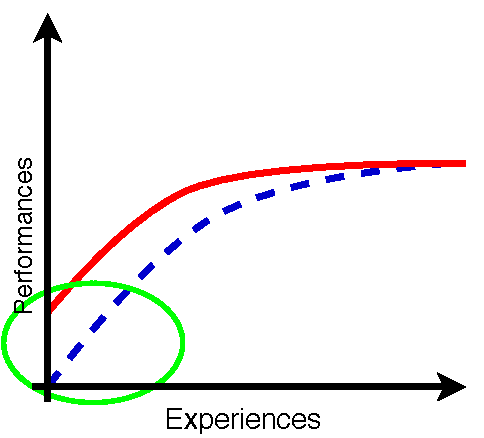
\includegraphics[width=0.3\textwidth]{objectives-jumpstart}
                    \label{fig:objectives-jumpstart}
                }
                \subfloat[Learning]{
                    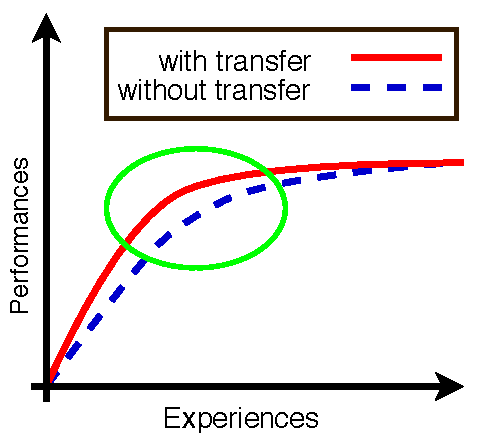
\includegraphics[width=0.3\textwidth]{objectives-learn}
                    \label{fig:objectives-learn}
                }
                \subfloat[Asymptotical]{
                    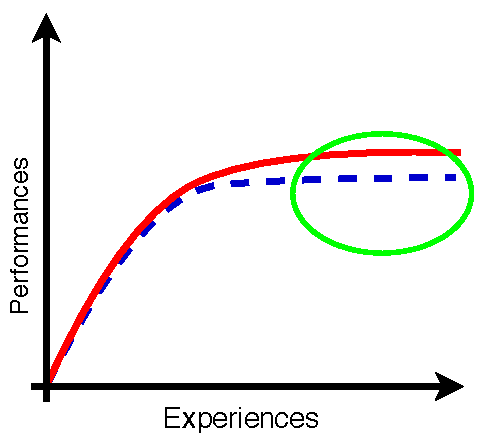
\includegraphics[width=0.3\textwidth]{objectives-asymptote}
                    \label{fig:objectives-asymptote}
                }
                \caption{Transfer learning objectives ~(Langley 2016)}
                \label{fig:objectives}
            \end{center}
        \end{figure}

    \end{frame}

    \begin{frame}{The settings}

        Two main setting:

        \begin{itemize}
            \item Domain $\cS\times \cA$ is not fixed. Find a mapping between a source and a target task.
            \item Domain is fixed:
            \begin{itemize}
                \item mono-task (one to one),
                \item generic-task (one to many),
                \item multi-task  (many to many).
            \end{itemize}
        \end{itemize}

    \end{frame}

    \begin{frame}{The knowledge transfered}

        Several types of knowledge:
        \begin{itemize}
            \item transitions ( ${(s_i,a_i,r'_i,s'_i)}_{i\in[0,N]}$ for example),
            \item representation (features, action space, options, reward shaping etc),
            \item parameters (meta parameters, Q-function, policy etc).
        \end{itemize}

    \end{frame}

    \begin{frame}{Negative Transfer}

        \begin{itemize}
            \item Transfer learning isn’t guaranteed to help
            \item Negative transfer occurs when performance is worse than learning
            target task from scratch (usually happen at the asymptote)
        \end{itemize}

    \end{frame}


    %%%%%%%%%%%%%%%%%%%%%%%%%%%%%%%%%%%%%%%%%%%%%%%%%%%%%%%%%%%%%%%
    %%%%%%%%%%%%%%%%%%%%%%%%%%%%%%%%%%%%%%%%%%%%%%%%%%%%%%%%%%%%%%%
    %%%%%%%%%%%%%%%%%%%%%%%%%%%%%%%%%%%%%%%%%%%%%%%%%%%%%%%%%%%%%%%
    %%%%%%%%%%%%%%%%%%%%%%%%%%%%%%%%%%%%%%%%%%%%%%%%%%%%%%%%%%%%%%%
    %%%%%%%%%%%%%%%%%%%%%%%%%%%%%%%%%%%%%%%%%%%%%%%%%%%%%%%%%%%%%%%
    %%%%%%%%%%%%%%%%%%%%%%%%%%%%%%%%%%%%%%%%%%%%%%%%%%%%%%%%%%%%%%%


    \section{Scaling TL}

    \begin{frame}
        Online learning and transfer for user adaptation in dialogue systems [Carrara et al. 2017, Sigdial]
    \end{frame}

    \subsection{Workflow}

    \foreach \n in {1,2,3,4,5,6,7,8,9,10,11,12}{
        \begin{frame}{Workflow}
            \begin{figure}
                \begin{center}
                    \includegraphics[width=0.75\textwidth]{dataflowRobot\n.pdf}
                \end{center}
            \end{figure}
        \end{frame}
    }


    \begin{frame}{Sources election | \textsc{PD-distance}}
        \begin{figure}
            \begin{center}
                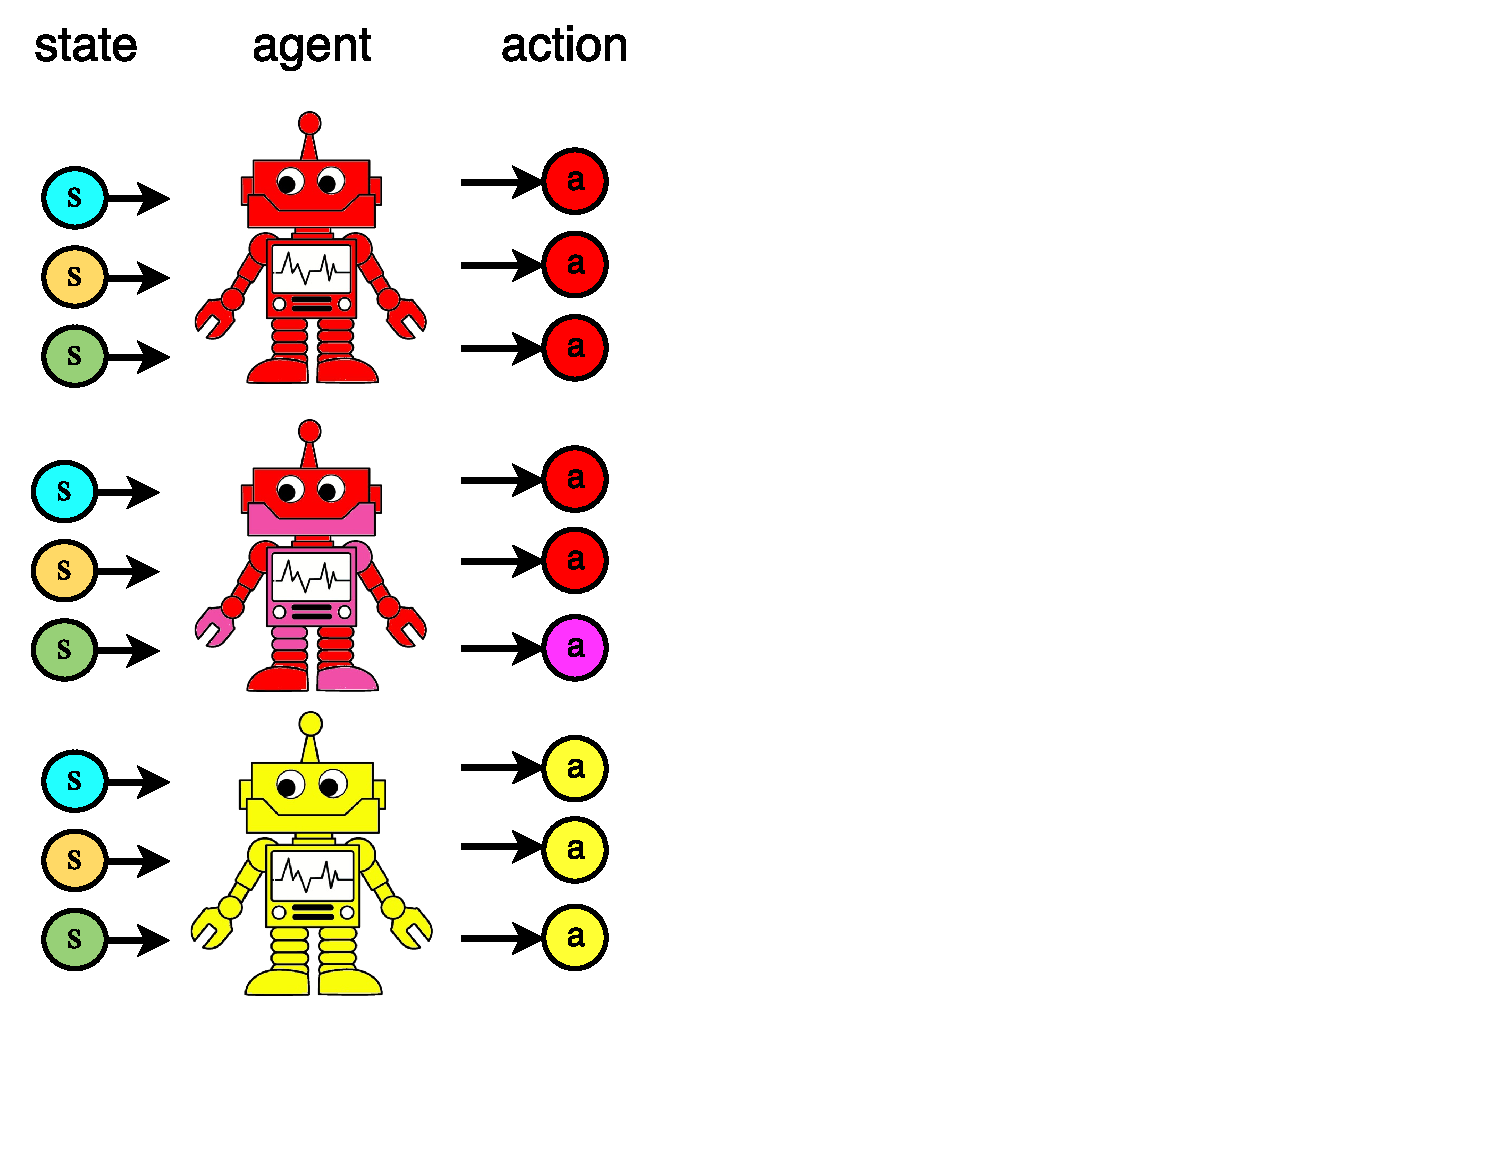
\includegraphics[width=0.8\textwidth]{pddistance0.pdf}
            \end{center}
        \end{figure}
    \end{frame}

    \begin{frame}{Sources election | \textsc{PD-distance}}
        \begin{figure}
            \begin{center}
                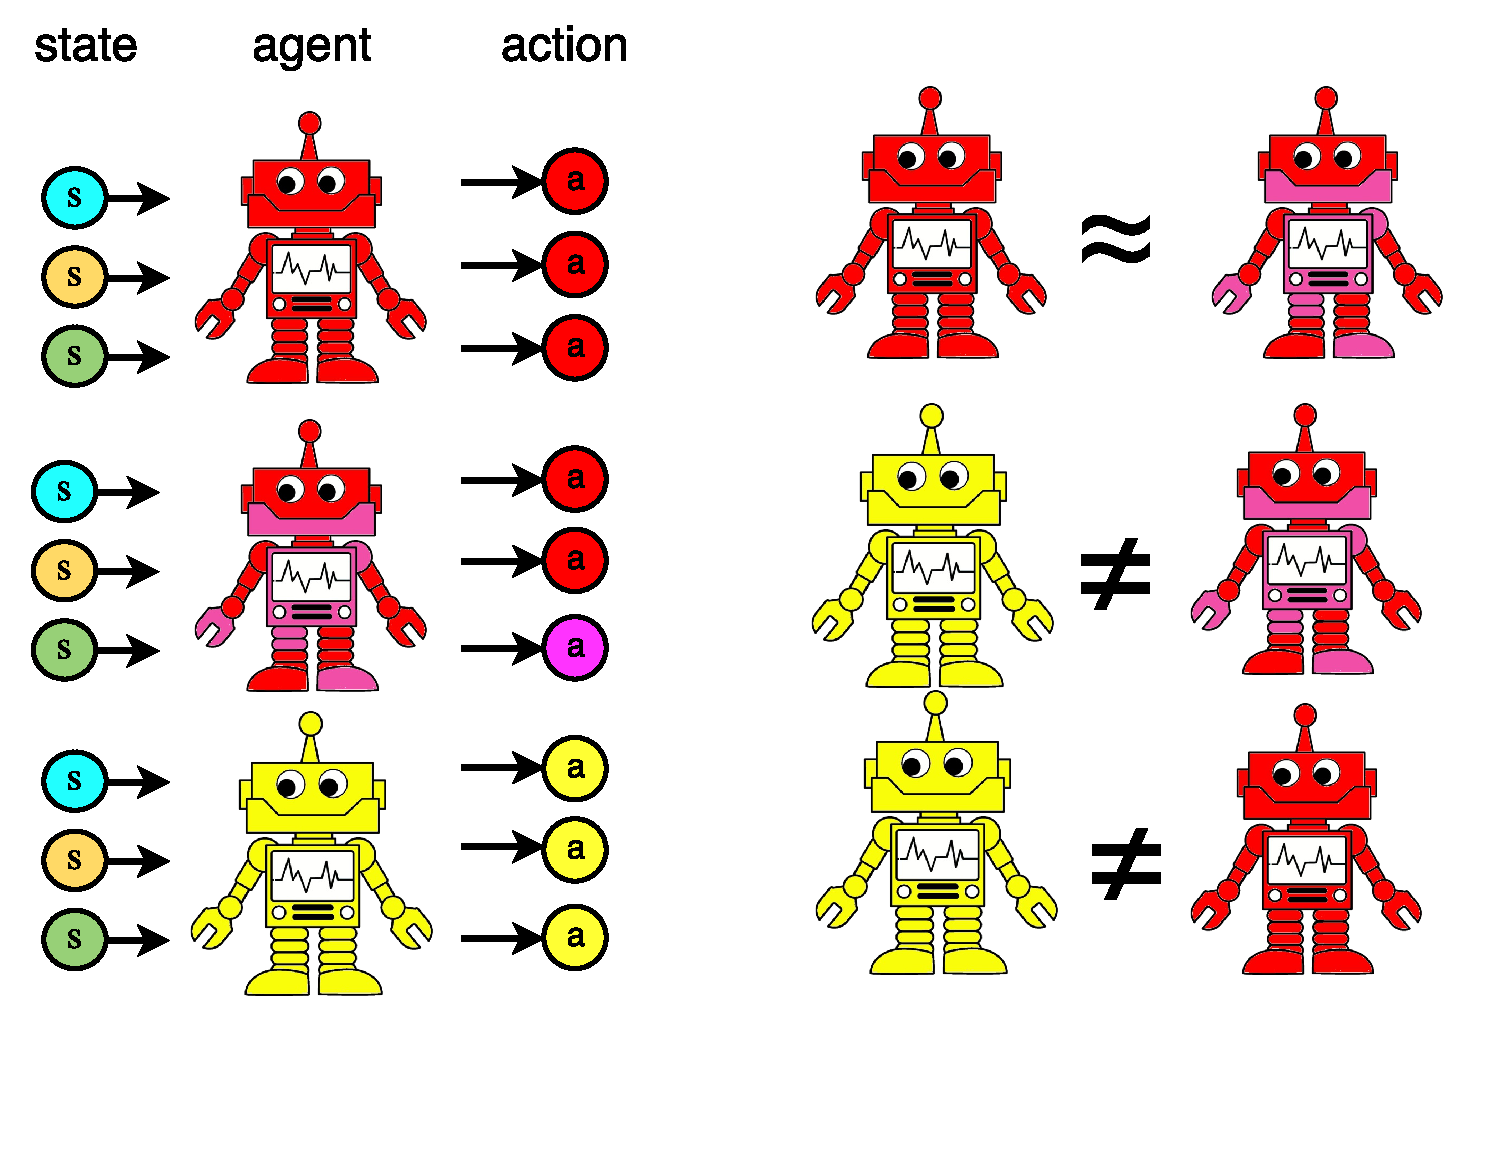
\includegraphics[width=0.8\textwidth]{pddistance.pdf}
            \end{center}
        \end{figure}
    \end{frame}
    \foreach \n in {0,1,2,3,4}{
        \begin{frame}{Sources election | \textsc{PD-distance}}
            \begin{figure}
                \begin{center}
                    \includegraphics[width=0.8\textwidth]{euclide\n.pdf}
                \end{center}
            \end{figure}
        \end{frame}
    }

    \begin{frame}{Sources election | \textsc{K-means}}
        \begin{figure}
            \begin{center}
                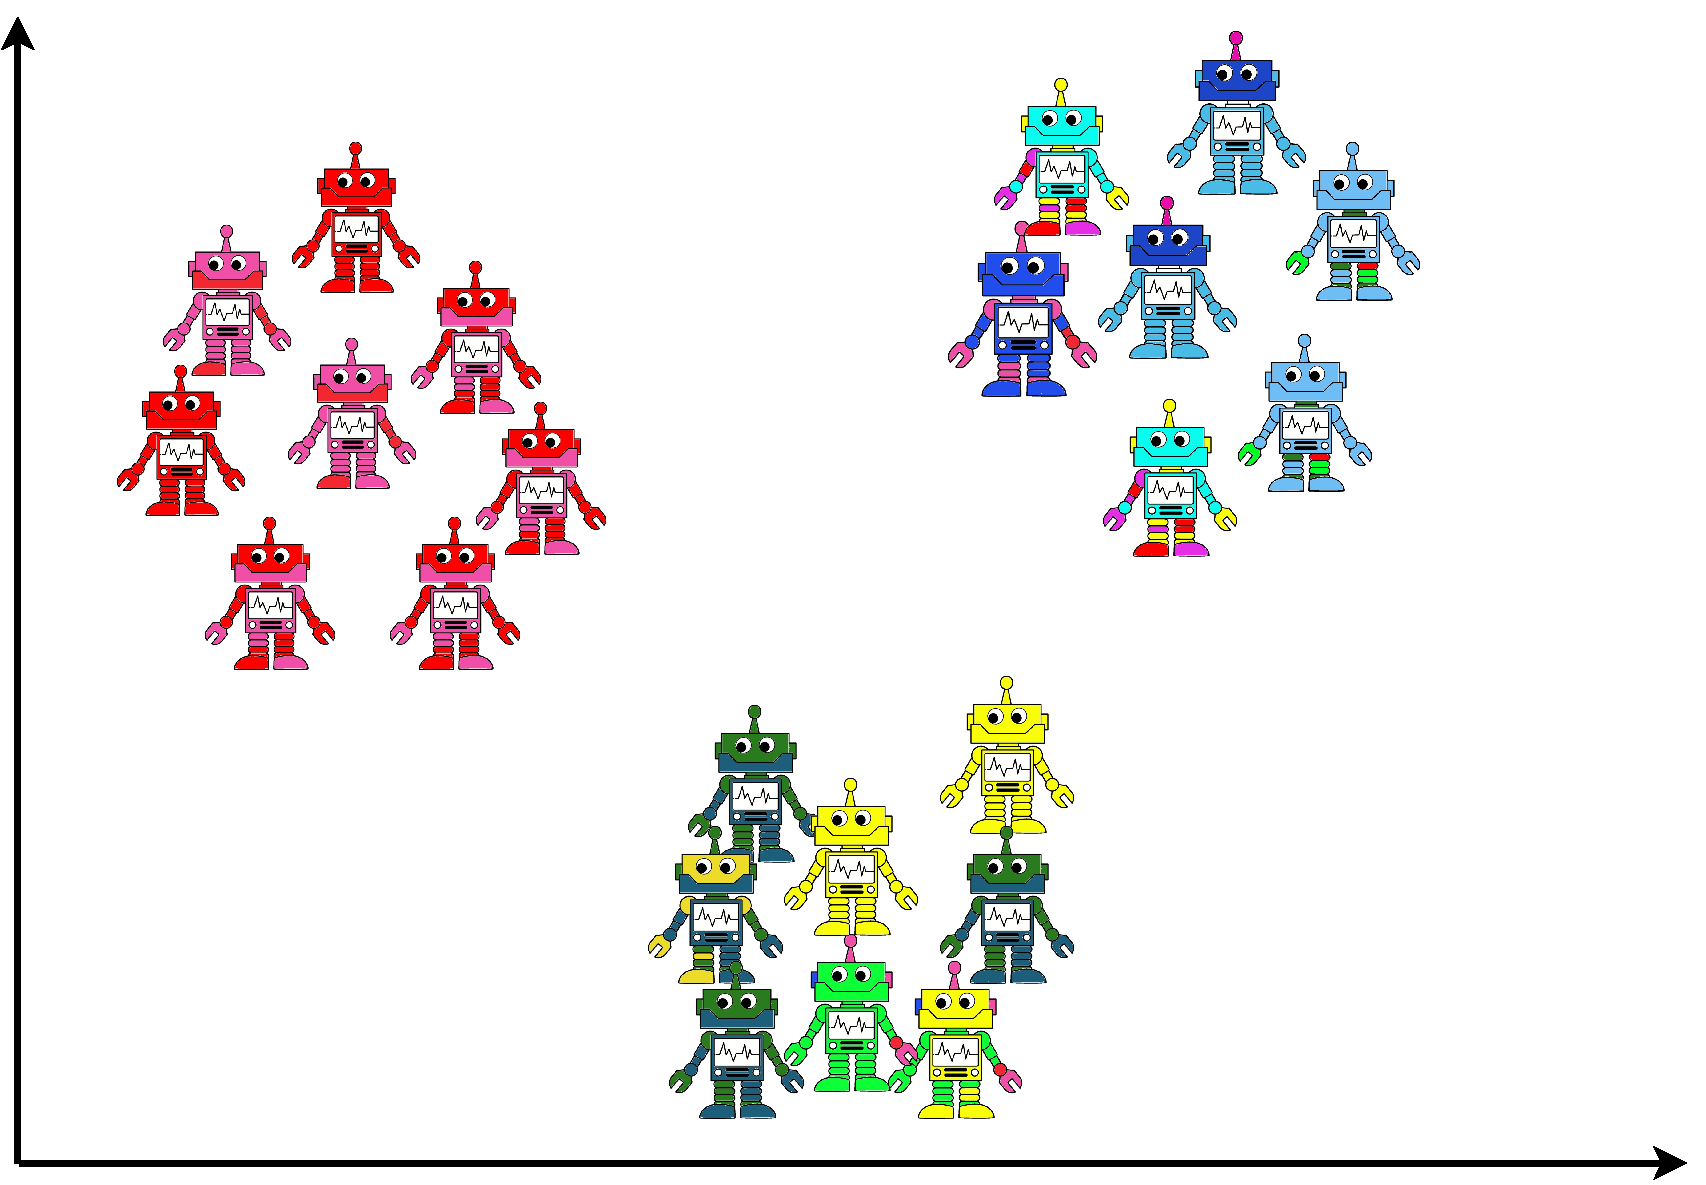
\includegraphics[width=0.8\textwidth]{clustering.pdf}
            \end{center}
        \end{figure}
    \end{frame}

    \foreach \n in {0}{
        \begin{frame}{Sources election |\textsc{K-means}}
            \begin{figure}
                \begin{center}
                    \includegraphics[width=0.8\textwidth]{kmeans\n.pdf}
                \end{center}
            \end{figure}
        \end{frame}
    }
    \begin{frame}{Sources election | \textsc{K-medoids}}
        \begin{figure}
            \begin{center}
                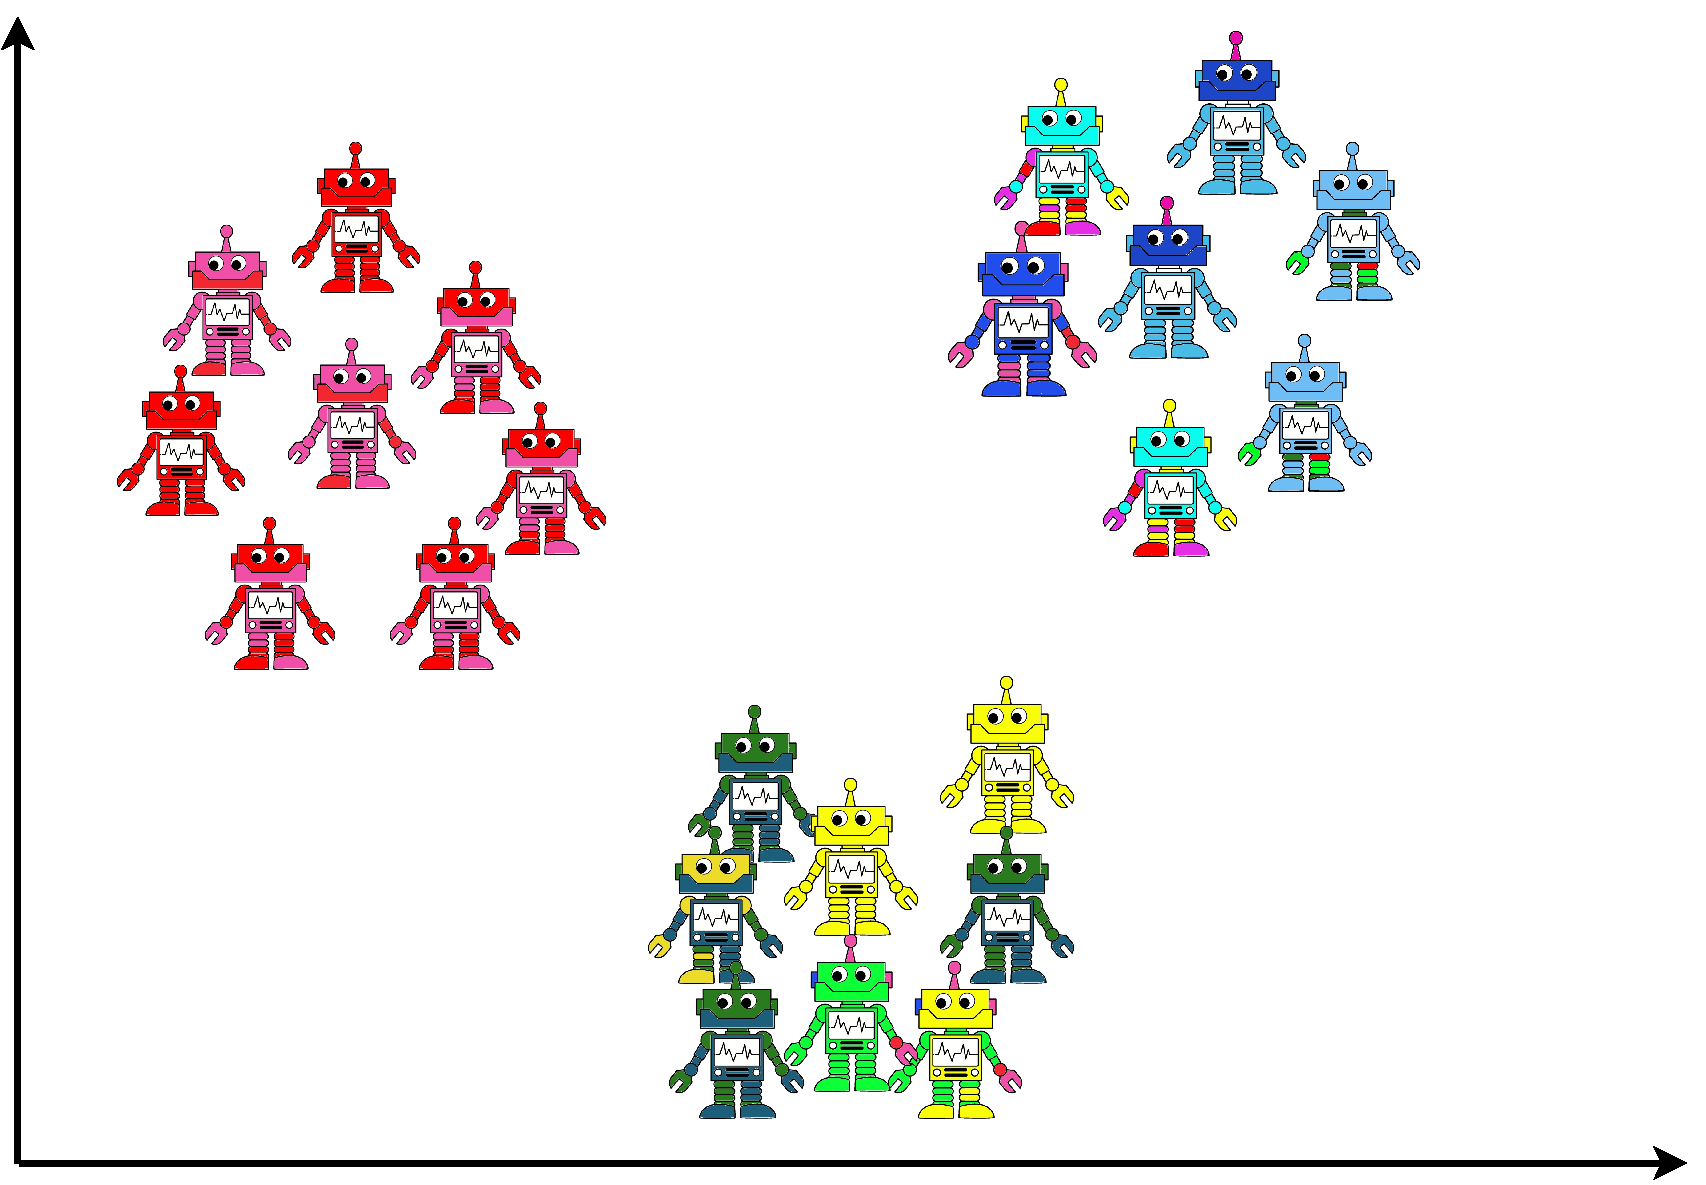
\includegraphics[width=0.8\textwidth]{clustering.pdf}
            \end{center}
        \end{figure}
    \end{frame}

    \begin{frame}{Sources election | \textsc{K-medoids}}
        \begin{figure}
            \begin{center}
                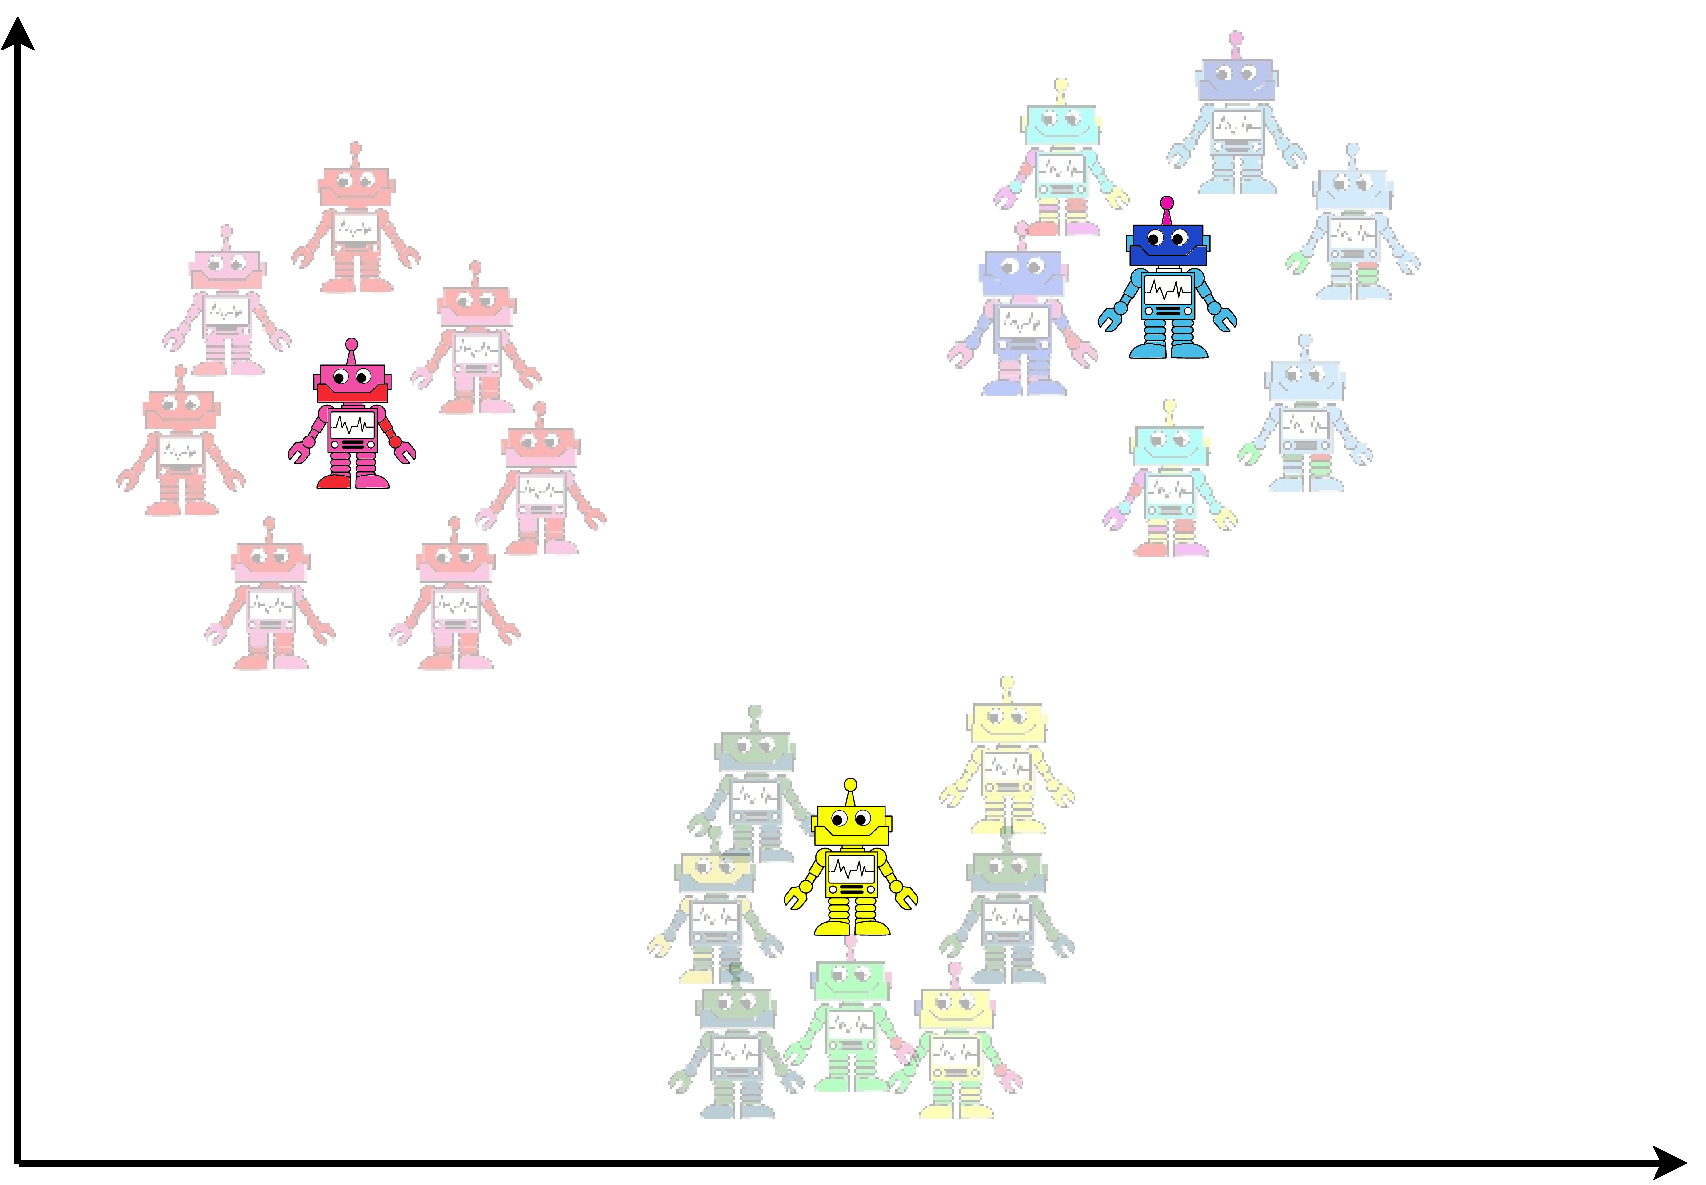
\includegraphics[width=0.8\textwidth]{kmedoids.pdf}
            \end{center}
        \end{figure}
    \end{frame}

    \foreach \n in {8}{
        \begin{frame}{Source selection | UCB1}
            \begin{figure}
                \begin{center}
                    \includegraphics[width=0.65\textwidth]{bd\n.pdf}
                \end{center}
            \end{figure}
        \end{frame}
    }

    \foreach \n in {0,1,2,3,4,5,6}{
        \begin{frame}{Transfer and Learning}
            \begin{figure}
                \begin{center}
                    \includegraphics[width=1.0\textwidth]{tftq\n.pdf}
                \end{center}
            \end{figure}
        \end{frame}
    }

    \subsection{Experiments}
    \begin{frame}{Simulated users}
        \begin{figure}
            \captionsetup[subfigure]{labelformat=empty}
            \begin{center}
                \subfloat[Overall score ]{
                    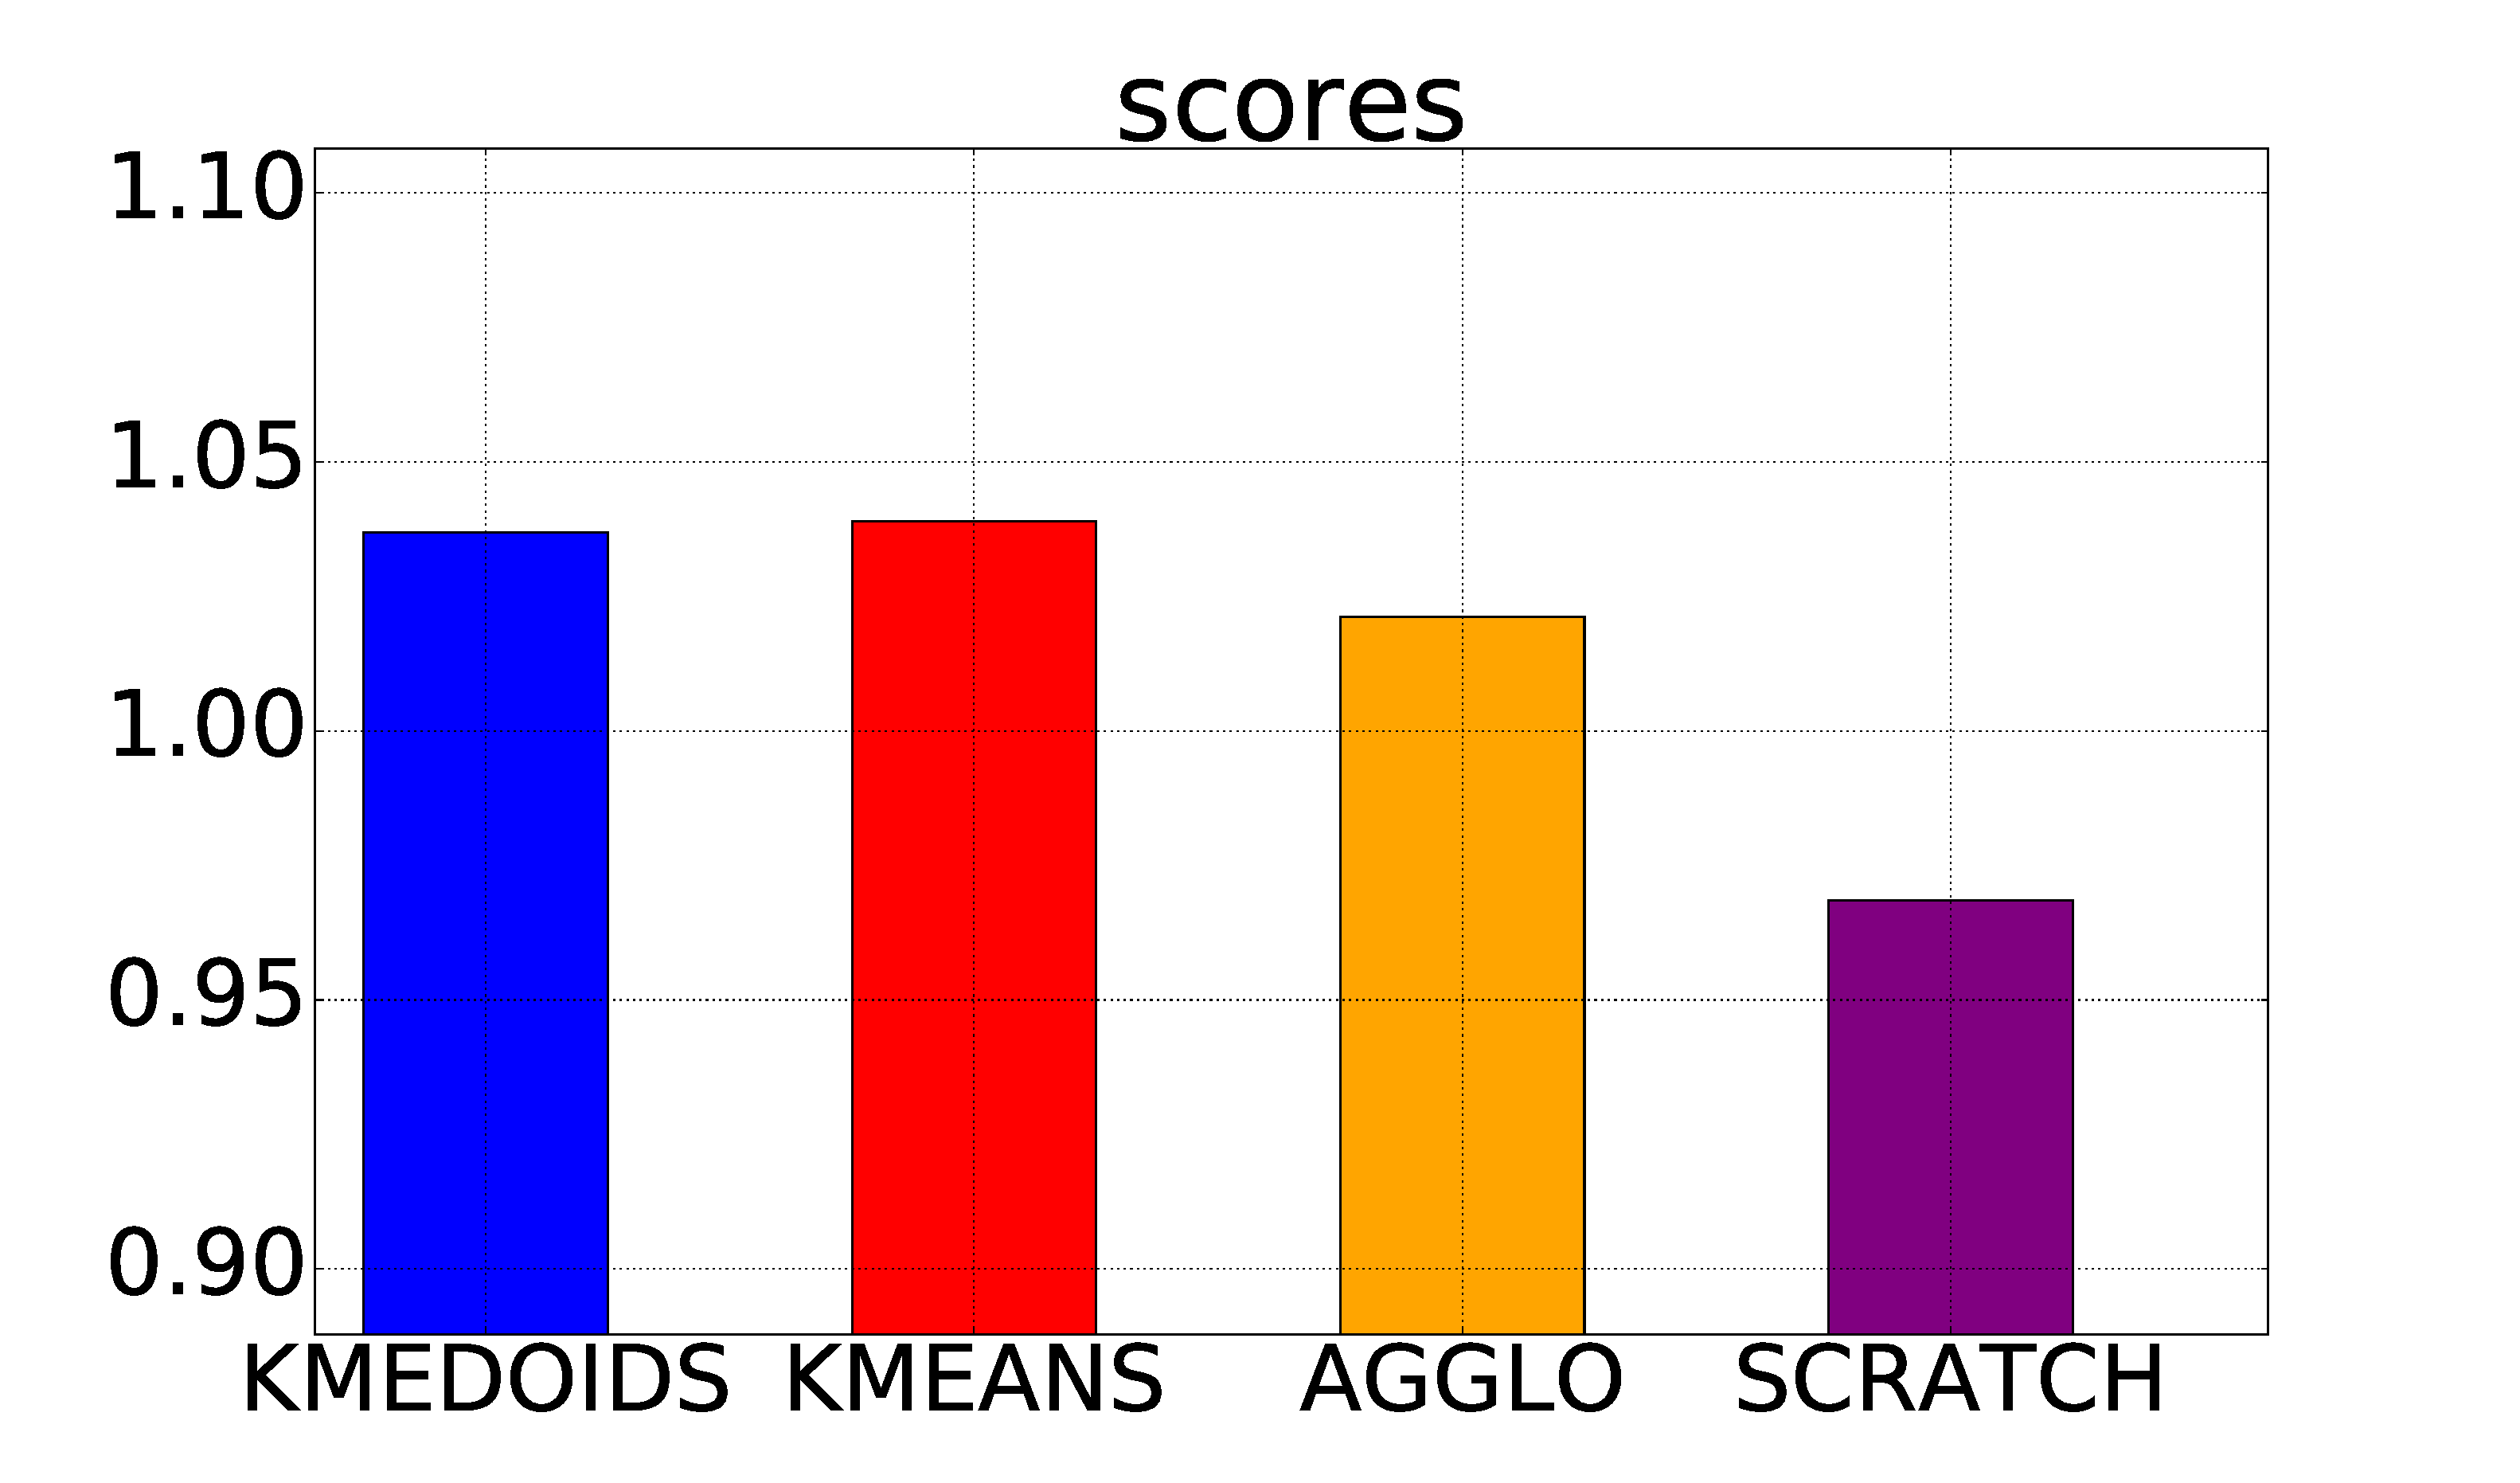
\includegraphics[width=0.5\textwidth]{img/handcraftedScores.pdf}
                }
                \subfloat[Dialogue size]{
                    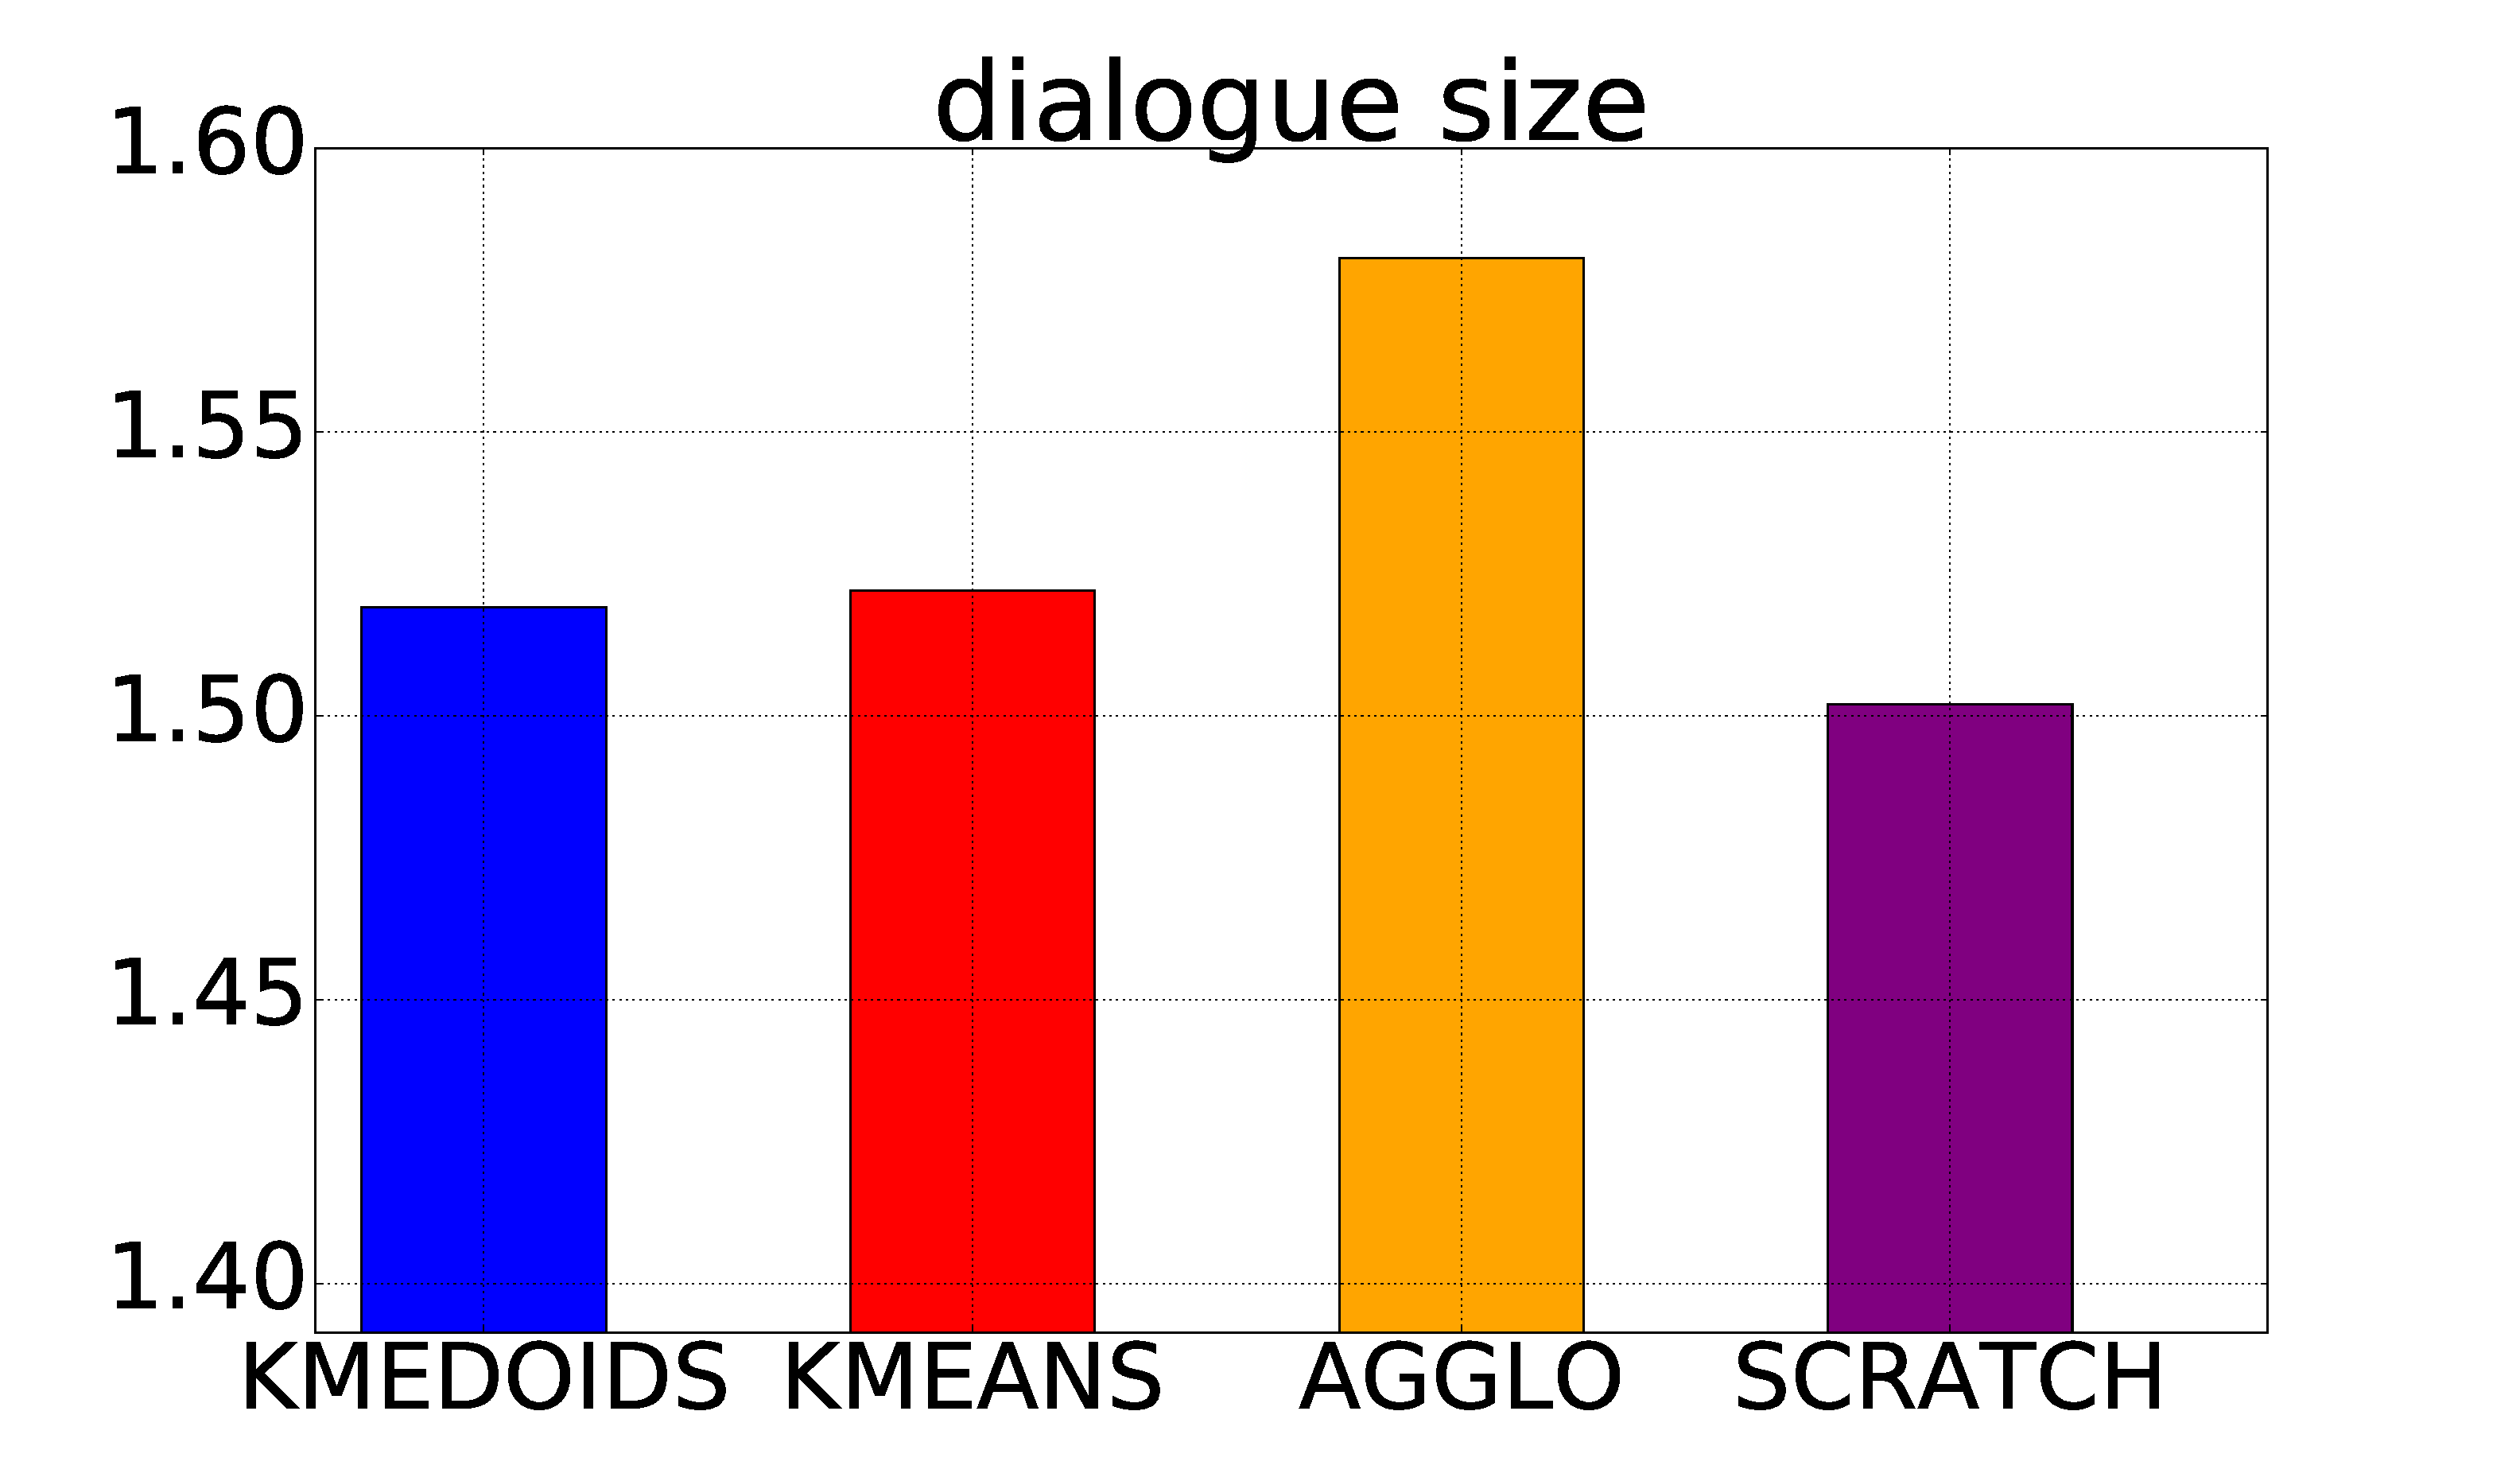
\includegraphics[width=0.5\textwidth]{img/handcraftedDialoguesize.pdf}
                }
            \end{center}
        \end{figure}
    \end{frame}

    \begin{frame}{Human-model users}
        \begin{figure}
            \captionsetup[subfigure]{labelformat=empty}
            \begin{center}
                \subfloat[Overall score ]{
                    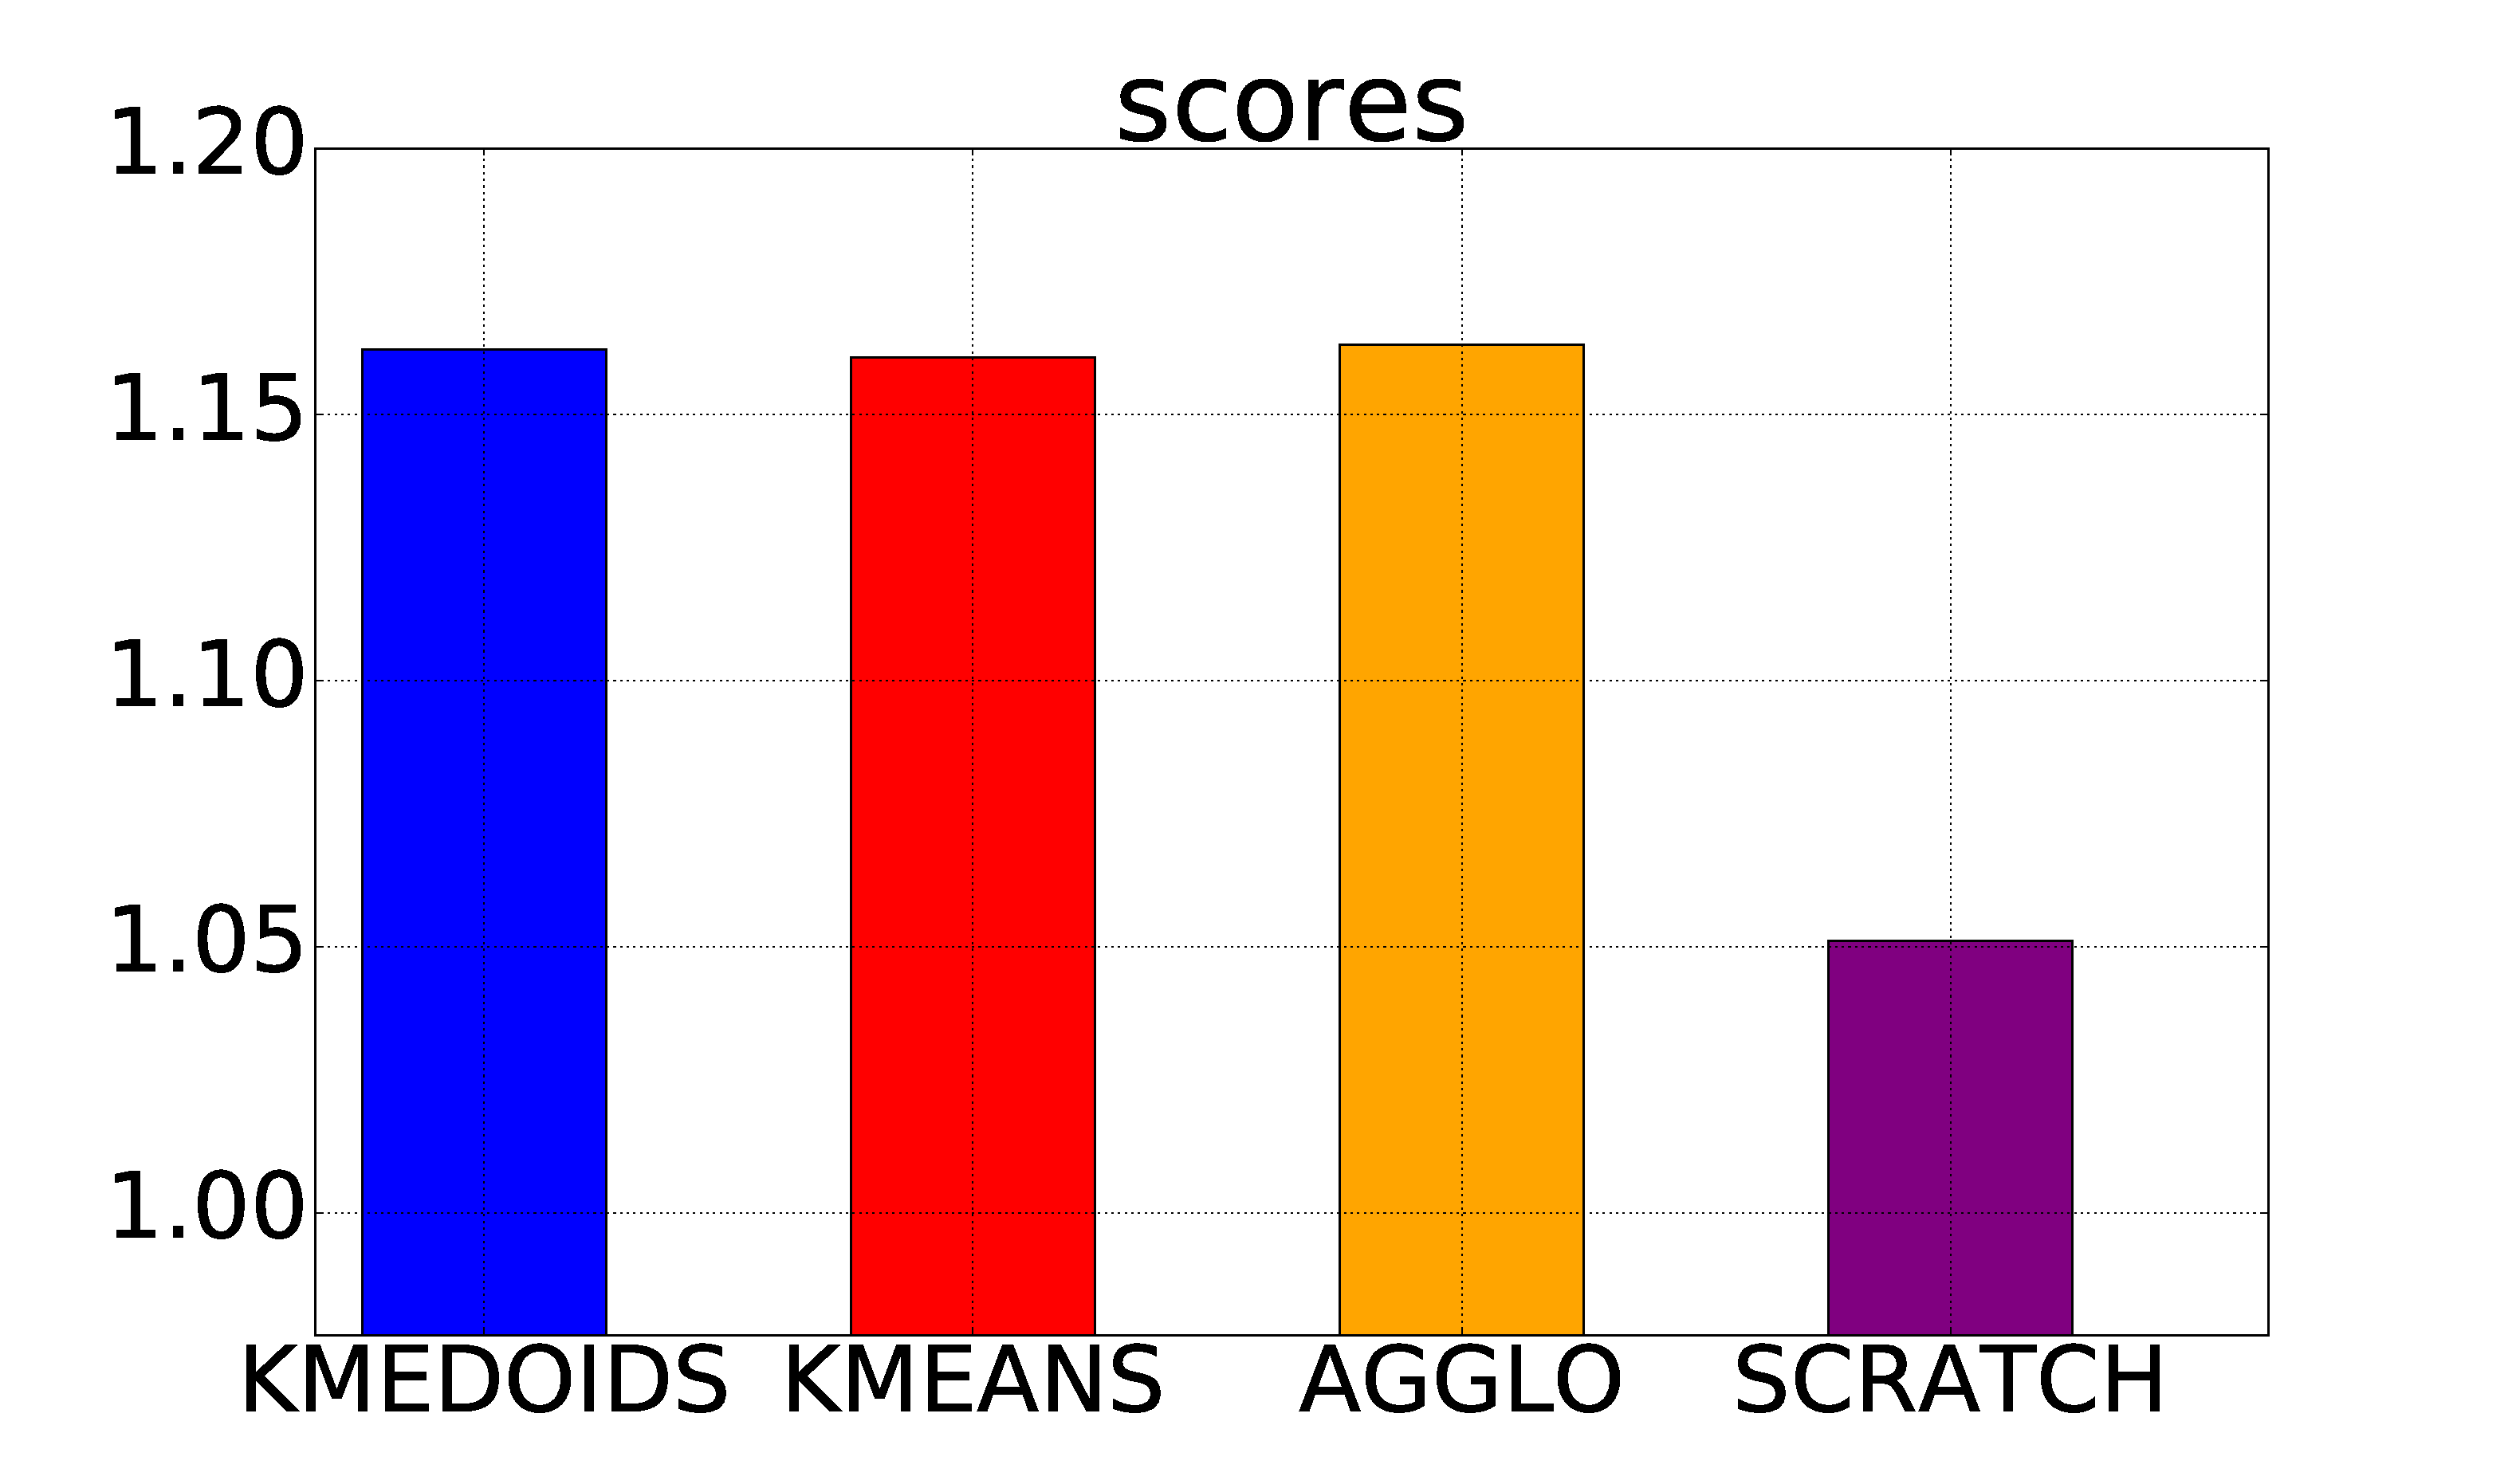
\includegraphics[width=0.5\textwidth]{img/humanScores.pdf}
                }
                \subfloat[Dialogue size]{
                    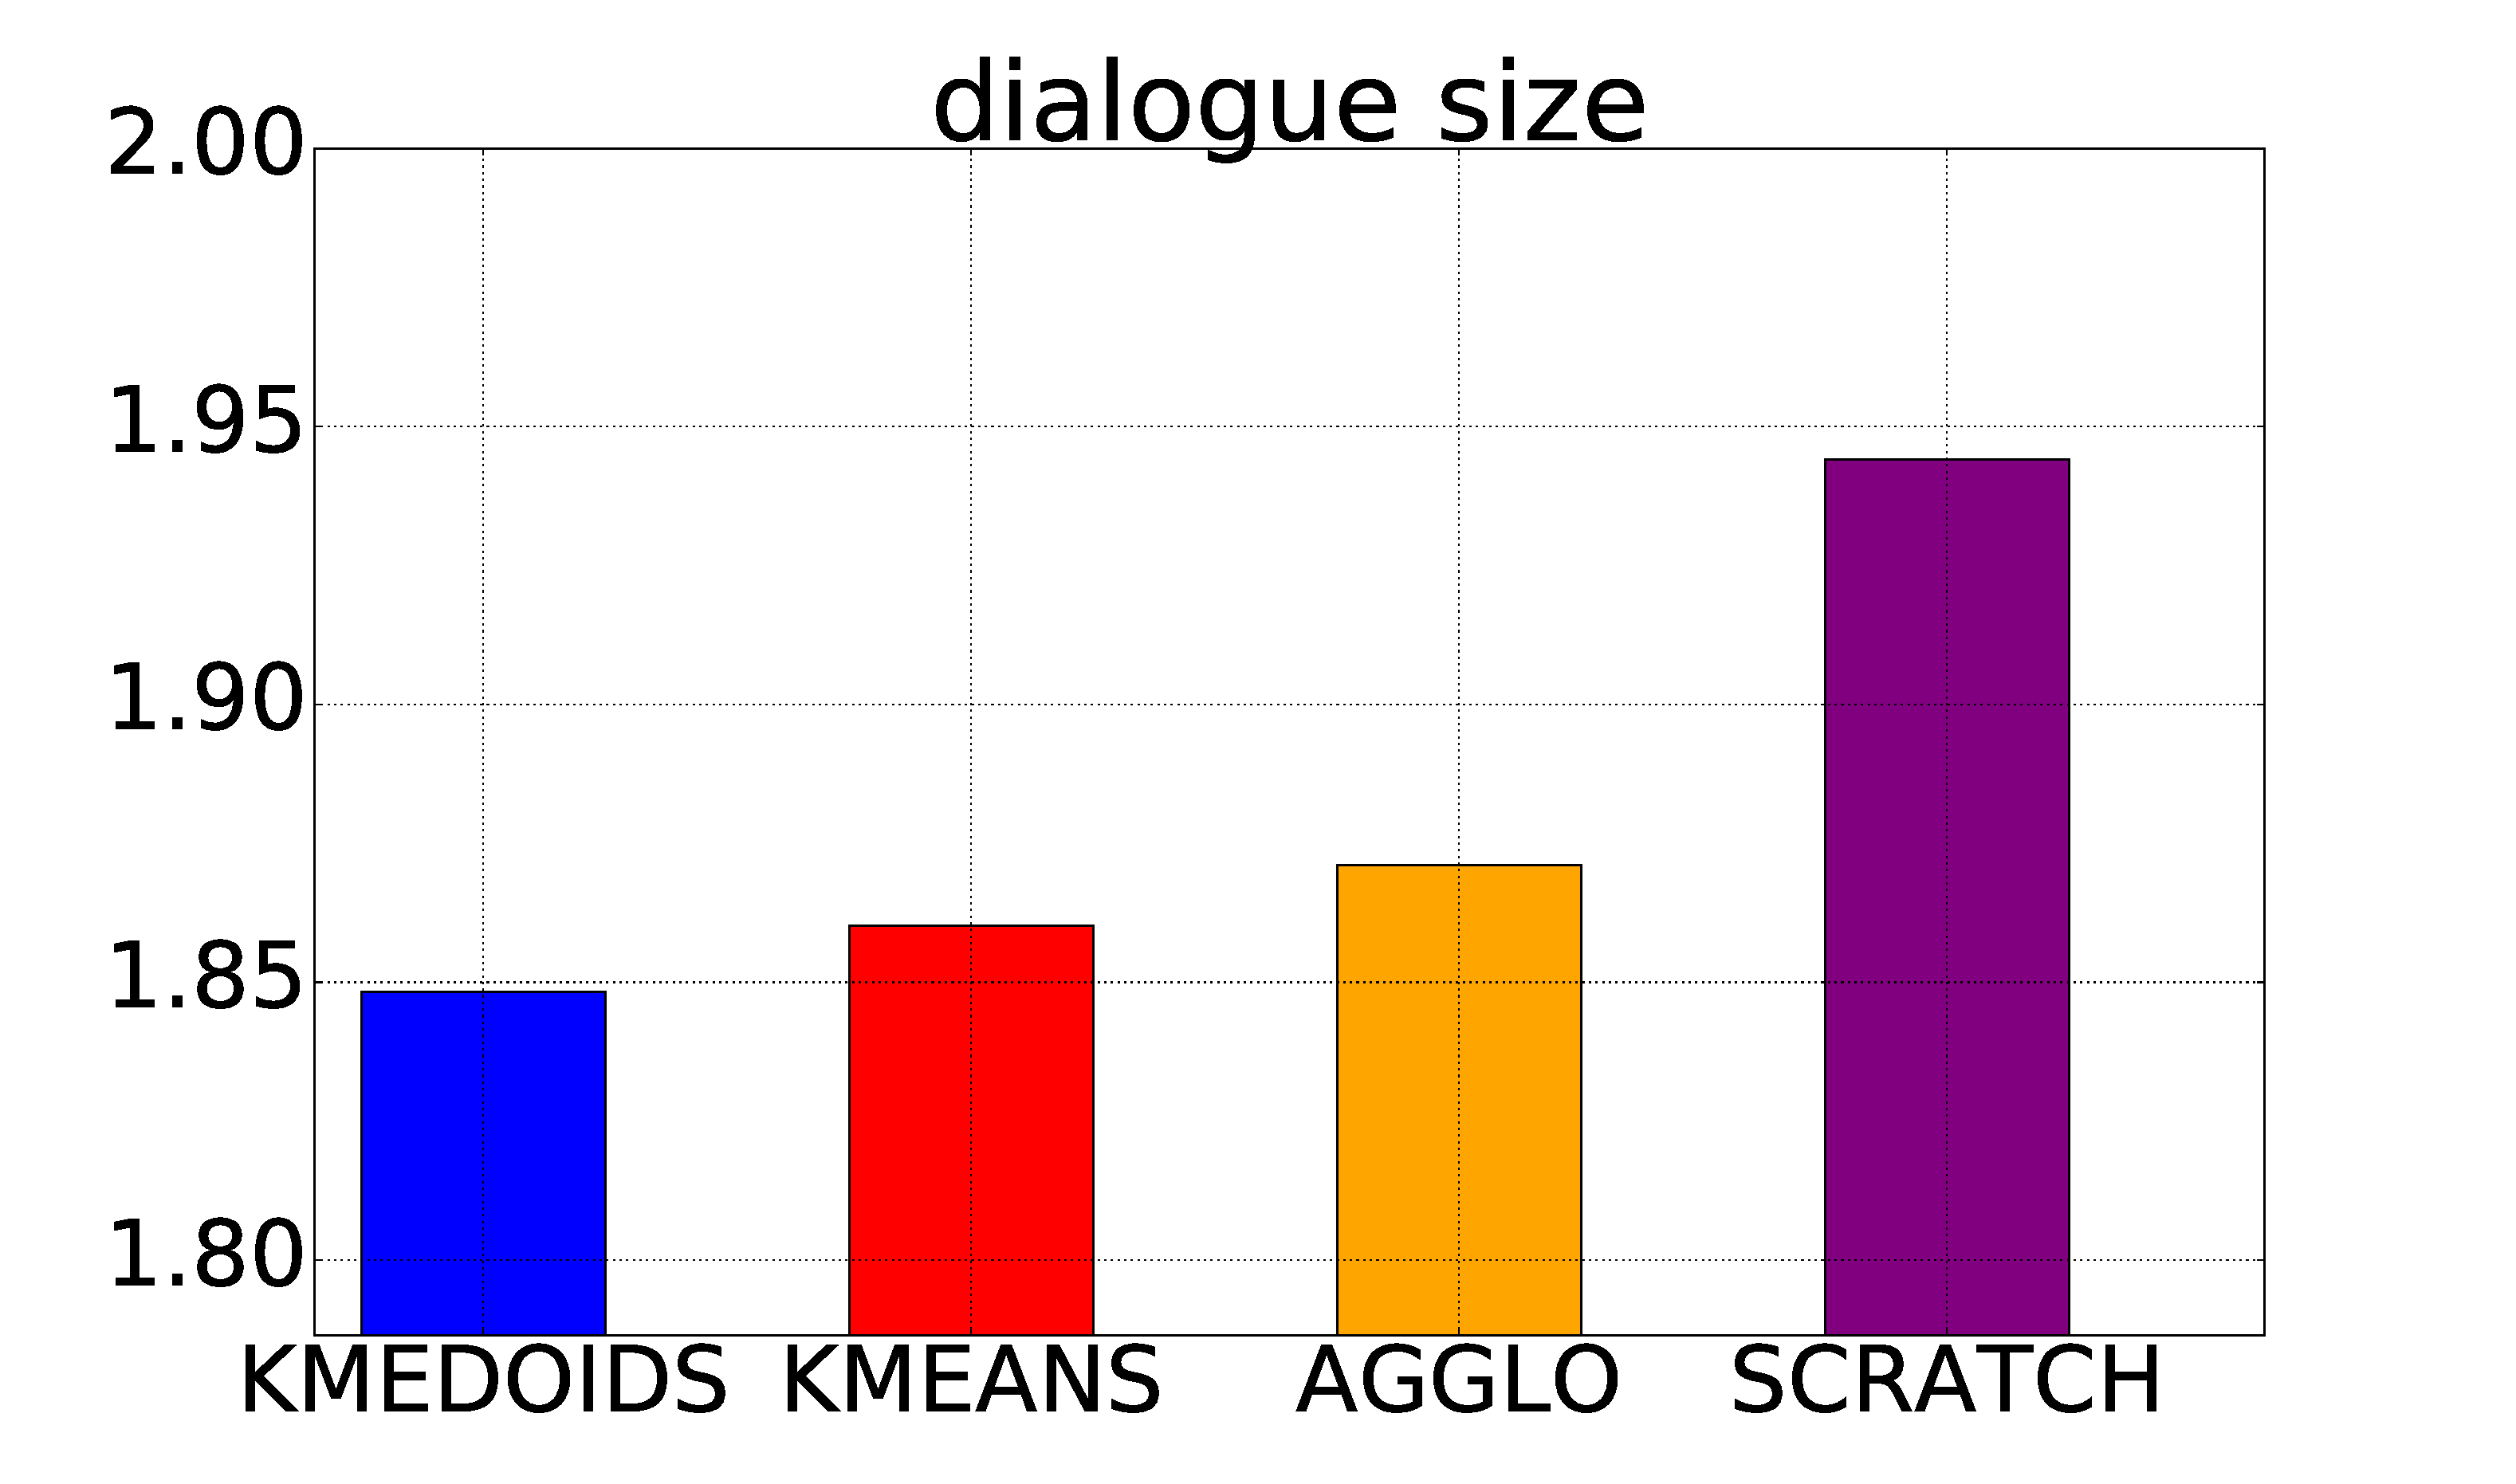
\includegraphics[width=0.5\textwidth]{img/humanDialoguesize.pdf}
                }
            \end{center}
        \end{figure}
    \end{frame}


    %%%%%%%%%%%%%%%%%%%%%%%%%%%%%%%%%%%%%%%%%%%%%%%%%%%%%%%%%%%%%%%%
    %%%%%%%%%%%%%%%%%%%%%%%%%%%%%%%%%%%%%%%%%%%%%%%%%%%%%%%%%%%%%%%%
    %%%%%%%%%%%%%%%%%%%%%%%%%%%%%%%%%%%%%%%%%%%%%%%%%%%%%%%%%%%%%%%%
    %%%%%%%%%%%%%%%%%%%%%%%%%%%%%%%%%%%%%%%%%%%%%%%%%%%%%%%%%%%%%%%%


    \section{Safe TL}

    \begin{frame}
        Budgeted RL for Continuous State Space
        [Carrara et al. 2019, NeurIPS]
    \end{frame}

    \subsection{A transfer problem}

    \begin{frame}

        \begin{alertblock}{Limitation}
            New tasks $\rightarrow$ requiere caution sometimes.
        \end{alertblock}

        \pause
        \begin{exampleblock}{Solution}
            \begin{itemize}
                \item Learning the policy for the target task,
                \item using a safe policy.
                \begin{itemize}
                    \item Notion of budget $\beta$: the average amount of risk allowed.
                \end{itemize}
            \end{itemize}
        \end{exampleblock}
        \pause
        \begin{block}{}
            How to learn this safe policy ?
        \end{block}

    \end{frame}

    \subsection{Mastering the risk in RL}

    \begin{frame}

        \begin{block}{Constraint}
            $C:S\times A \rightarrow \{0,1\}$.
        \end{block}
        \pause
        \begin{block}{Lagragian relaxation}
            $R \leftarrow R - \lambda C$.
        \end{block}

        \pause
        \begin{alertblock}{Limitation}
            What $\lambda$ for what budget $\beta$?
        \end{alertblock}
        \pause
        \begin{exampleblock}{Solution: $\lambda$ calibration}% oral: limitation des politiques lagragiennes
            Searching the safe policy on the Pareto front.
        \end{exampleblock}


    \end{frame}

    \foreach \n in {0,1}{
        \begin{frame}{}
            \begin{figure}
                \begin{center}
                    \includegraphics[width=1\textwidth]{pareto\n.pdf}
                \end{center}
            \end{figure}
        \end{frame}
    }

    \begin{frame}
        \begin{alertblock}{Limitations}
            \begin{itemize}
                \item \cmoins Cumbersome and not reliable processus.  % où commencer, quel steps ?
                \item \cmoins It is possible that no $\lambda$ exists for $\beta$.
                \item \cmoins Deterministics policies $\rightarrow$ extreme behaviours.
                % pas de formulation linéaire de la reward pour un budget donné
            \end{itemize}
        \end{alertblock}
        \pause
        \begin{exampleblock}{Solution}
            Budgeted Reinforcement Learning.
            % Ce qui nous amène à la prochaine contribution: BRL
        \end{exampleblock}
    \end{frame}

    \subsection{MDP}

    \begin{frame}{Framework}
        \begin{block}{Markov Decision Processes (MDP)}
            \begin{itemize}
                \item $(\cS, \cA, P, R, \gamma)$
                \item $G_r^\pi = \sum_{t=0}^\infty \gamma^t R(s_t, a_t)$ return of rewards.
                \item Find $\pi^*$ s.t $\forall s\in\cS$:
                \begin{equation}
                    \label{eq:mdp}
                    \begin{array}{lcr}
                        \displaystyle \pi^* \in \argmax_{\pi\in\cM(\cA)^\cS} \expectedvalue[G_r^\pi | s_0=s]
                    \end{array}
                \end{equation}

            \end{itemize}
        \end{block}


        \begin{block}{}
            \begin{itemize}
                \item \cplus \textit{Tractable}.
                \item \cmoins Extreme behaviours.
                \item \cmoins Need calibration (which $\lambda$ for $\beta$?).
                % A l ORAL si formulation sous contrainte
            \end{itemize}
        \end{block}

    \end{frame}

    \subsection{CMDP}

    \begin{frame}{Framework}

        \begin{block}{\textcolor{purple}{Constrained} Markov Decision Processes (CMDP)}
            \begin{itemize}
                \item $(\cS, \cA, P, R,\textcolor{purple}{C}, \gamma,\textcolor{purple}{\beta})$
                \item $G_r^\pi = \sum_{t=0}^\infty \gamma^t R(s_t, a_t)$ return of rewards.
                \item \textcolor{purple}{ $G_c^\pi = \sum_{t=0}^\infty \gamma^t C(s_t, a_t)$ return of costs.}
                \item Find $\pi^*$ s.t $\forall s\in\cS$:
                \begin{equation}
                    \label{eq:cmdp}
                    \begin{array}{lcr}
                        \displaystyle \pi^* \in \argmax_{\pi\in\cM(\cA)^\cS} \expectedvalue[G_r^\pi | s_0=s] \\
                        \text{ s.t. }  \textcolor{purple}{\expectedvalue[G_c^\pi | s_0=s] \leq \beta}
                    \end{array}
                \end{equation}
            \end{itemize}
        \end{block}

        \begin{block}{}
            \begin{itemize}
                \item \cplus \textit{Tractable}.
                \item \cmean add a DOF (if policies mixtures).% A L ORAL On peut définir un budget de safety , formuation plus naturelle
                \item \cmoins fixed budged.
                % A L ORAL si le budget change on the fly, ou qu'il n'est pas adapté, on doit reapprendre une politique,  Or Le front de pareto est rarement linéaire, le choix du budget n'est pas évident


            \end{itemize}
        \end{block}

    \end{frame}

    \subsection{BMDP}

    \begin{frame}{Framework}

        \begin{block}{\textcolor{purple}{Budgeted} Markov Decision Process (BMDP)}
            \begin{itemize}
                \item $(\cS, \cA, P, R,{C}, \gamma,\textcolor{purple}{\cB})$
                \item $G_r^\pi = \sum_{t=0}^\infty \gamma^t R(s_t, a_t)$ return of rewards.
                \item  $G_c^\pi = \sum_{t=0}^\infty \gamma^t C(s_t, a_t)$ return of costs.
                \item Find $\pi^*$ s.t $\forall (s,\textcolor{purple}{\beta})\in\cS\times\textcolor{purple}{\cB}$:
                \begin{equation}
                    \label{eq:bmdp}
                    \begin{array}{lcr}
                        \displaystyle \pi^* \in \argmax_{\pi\in\cM(\cA\times\textcolor{purple}{\cB})^{\cS\times\textcolor{purple}{\cB}}} \expectedvalue[G_r^\pi | s_0=s,\textcolor{purple}{\beta_0=\beta}] \\
                        \text{ s.t. }  \expectedvalue[G_c^\pi | s_0=s,\textcolor{purple}{\beta_0=\beta}] \leq \beta
                    \end{array}
                \end{equation}
            \end{itemize}
        \end{block}


        \begin{block}{}
            \begin{itemize}
                \item \cmoins \textit{Untractable}.
                \item \cplus add a DOF.
                \item \cplus unfixed budget.

                % A L ORAL On peut définir un budget de safety et d'afranchir des lambda.}
            \end{itemize}
        \end{block}

    \end{frame}


    \begin{frame}{Augmented settings}

        \textbf{Budgeted Policies} $\pi\in\Pi$
        \begin{itemize}
            \item $ \pi:\underbrace{(s,\beta)}_{\os} \rightarrow \underbrace{(a,\beta')}_{\oa}$
        \end{itemize}

        \textbf{Domain}
        \begin{itemize}
            \item State $\ocS = \cS\times\cB$.
            \item Actions $\ocA = \cA\times\cB$.
            \item Dynamic $\ov{P}$
            %$\left((s',\beta') \condbar (s,\beta), (a, \beta_a)\right) \eqdef P(s'|s, a)\delta(\beta' - \beta_a)$.
        \end{itemize}
        \textbf{2D signals}
        \begin{itemize}
            \item Rewards $\ov{R} = (R, C)$
            \item Returns $G^\pi = (G_r^\pi, G_c^\pi)$
            \item $V^\pi(\os) = (V_r^\pi, V_c^\pi) \eqdef \expectedvalue\left[ G^\pi \condbar \ov{s_0} = \os\right]$
            \item $Q^\pi(\os, \oa)= (Q_r^\pi, Q_c^\pi) \eqdef \expectedvalue\left[ G^\pi \condbar \ov{s_0} = \os, \ov{a_0} = \oa\right]$
        \end{itemize}

    \end{frame}

    \begin{frame}{Optimality}
        \begin{definition}
            \begin{enumerate}
                \item[(i)] \pause\colorbox{red}{Respect the budget $\beta$}:
                \begin{equation*}
                    \Pi_a(\os) \eqdef \{\pi\in\Pi: V_c^\pi(s, \beta) \mathcolorbox{red}{\leq \beta}\}
                \end{equation*}
                \item[(ii)] \pause\colorbox{green}{Maximise rewards}:
                \begin{equation*}
                    V_r^*(\os) \eqdef \mathcolorbox{green}{\max}_{\pi\in\Pi_a(\os)}  V_r^\pi(\os) \qquad\quad \Pi_r(\os) \eqdef \mathcolorbox{green}{\argmax}_{\pi\in\Pi_a(\os)}  V_r^\pi(\os)
                \end{equation*}
                \item[(iii)] \pause\colorbox{yellow}{Minimise costs}:
                \begin{equation*}
                    V_c^*(\os) \eqdef \mathcolorbox{yellow}{\min}_{\pi\in\Pi_r(\os)}  V_c^\pi(\os), \qquad\quad \Pi^*(\os) \eqdef \mathcolorbox{yellow}{\argmin}_{\pi\in\Pi_r(\os)}  V_c^\pi(\os)
                \end{equation*}
            \end{enumerate}

            \pause We define $Q^*$ in the same fashion.
        \end{definition}
    \end{frame}

    \begin{frame}{}
        \begin{block}{Bellman optimality equation}
            $Q^*$ verifies:
            \begin{align*}
                Q^{*}(\os, \oa) &= \cT Q^{*}(\os, \oa)\\
                &\eqdef \ov{R}(\os, \oa) + \gamma \sum_{\os'\in\ocS} \ov{P}(\ov{s'} | \os, \oa)\sum_{\ov{a'}\in \ocA} \pi_\text{greedy}(\ov{a'}|\ov{s'}; Q^*) Q^{*}(\ov{s'}, \ov{a'}),
            \end{align*}
            with:\pause
            \begin{align*}
                \pi_\text{greedy}(\cdot|\os; Q) \in &\mathcolorbox{yellow}{\argmin}_{\rho\in\Pi_r^Q} \sum_{\oa}\rho(\oa) Q_c(\os, \oa), \\
                \text{where }\quad \Pi_r^Q \eqdef &\mathcolorbox{green}{\argmax}_{\rho\in\cM(\ocA)} \sum_{\oa}\rho(\oa) Q_r(\os, \oa) \\
                & \text{ s.t. }   \sum_{\oa}\rho(\oa) Q_c(\os, \oa) \mathcolorbox{red}{\leq \beta}
            \end{align*}
        \end{block}
        % ORAL: comment résoudre ce problème ?
    \end{frame}


    \foreach \n in {0,1,2,3,4}{
        \begin{frame}{Solving the non linear program}
            \begin{figure}
                \centering
                %%\vspace{-1.5em}
                \includegraphics[scale=1.0,page=1]{img/b\n}
            \end{figure}
        \end{frame}
    }

    \begin{frame}{Asymptotical behaviour}


        \begin{alertblock}{ \cmoins $\cT$ is not a contraction:}
            $\forall\epsilon>0, \exists Q^1,Q^2\in(\Real^2)^{\ocS\ocA}:\|\cT Q^1-\cT Q^2\|_\infty \geq \frac{1}{\epsilon}\|Q^1-Q^2\|_\infty$
        \end{alertblock}

        \begin{exampleblock}{\cplus unless $Q$-fonctions are smooth:}
            $\cT$ is a contraction for the subset $\cL_\gamma$ of $Q$-functions such that "$Q_r$ is $L$-Lipschitz w.r.t $Q_c$", with $L<\frac{1}{\gamma}-1$

        \end{exampleblock}
    \end{frame}

    \begin{frame}

        \begin{block}{Budgeted Value-Iteration}
            \begin{itemize}
                \item $Q \leftarrow \mathbf{0}$
                \item $Q(\os,\oa) \leftarrow \bo Q(\os,\oa)\ \forall (\os,\oa)$ jusqu'à convergence % peut ne pas arriver
                \item Return $\pi(\os) = \pi_\text{greedy}(\cdot|\os; Q)$
            \end{itemize}
        \end{block}
        \pause
        \begin{alertblock}{}
            \begin{itemize}
                \item How to compute $\bo Q$ if $\transition$, $\reward$ et $\constraint$ are unknown?
                \begin{itemize}
                    \item Sampling with $\mathcal{D}=\{(\os_i,\oa_i,\ov{r}_i',\os_i')\}_{i\in[0,N]}$
                \end{itemize}
                \item How to compute $Q\ \forall (\os,\oa) \in \ocS\times\ocA$ if $\ocS$ is large or continuous ?
                \begin{itemize}
                    \item Function approximation
                \end{itemize}
            \end{itemize}

        \end{alertblock}
        \pause
        \begin{block}{Budgeted Fitted-Q}
            \begin{itemize}
                \item $Q \leftarrow \mathbf{0}$
                \item $Q \leftarrow \Gamma(\{\os_{\indextransition},\oa_{\indextransition}\}_{{\indextransition}\in \T},\{\ov{r}'_{\indextransition} + \gamma \sum_{\ov{a}'\in \cA} \pi_\text{greedy}(\ov{a}'|\ov{s}'_{\indextransition}; Q) Q(\ov{s}'_{\indextransition}, \ov{a}')_{{\indextransition} \in \T}\})$
                \item Return $\pi(\os) = \pi_\text{greedy}(\cdot|\os; Q)$
            \end{itemize}
        \end{block}
    \end{frame}

    \subsection{Experiments}

    \begin{frame}{Dialogue systems}
        \begin{center}
            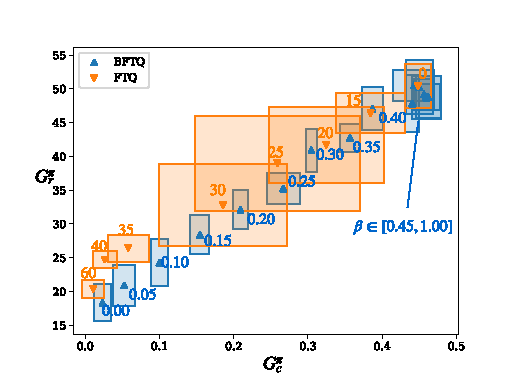
\includegraphics[scale=0.9]{img/slot-filling.pdf}
        \end{center}
    \end{frame}

    \begin{frame}{Autonomous driving}
        \begin{center}
            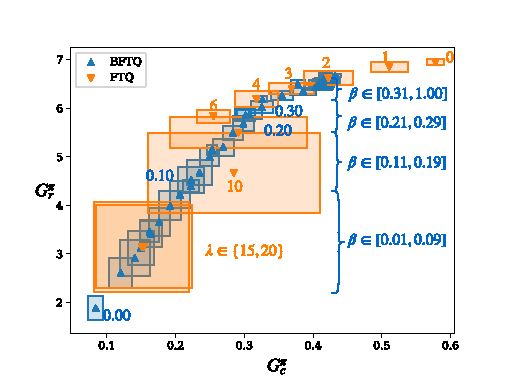
\includegraphics[scale=0.9]{img/highway.pdf}
        \end{center}
    \end{frame}

    \begin{frame}{Conclusion}
        \begin{itemize}
            \item Online RL is limited, especially if no simulator if available.
            \begin{itemize}
                \item Use Transfer Learning: transfer knowledge from source tasks to target tasks.
            \end{itemize}
            \item We have seen 2 methods:
            \begin{itemize}
                \item a pipeline that can handle a growing database of tasks,
                \item and a safe transfer learning framework for sensitive tasks.
            \end{itemize}
        \end{itemize}

    \end{frame}


\end{document}

